\documentclass[twoside]{book}

% Packages required by doxygen
\usepackage{calc}
\usepackage{doxygen}
\usepackage{graphicx}
\usepackage[utf8]{inputenc}
\usepackage{makeidx}
\usepackage{multicol}
\usepackage{multirow}
\usepackage{textcomp}
\usepackage[table]{xcolor}

% Font selection
\usepackage[T1]{fontenc}
\usepackage{mathptmx}
\usepackage[scaled=.90]{helvet}
\usepackage{courier}
\usepackage{amssymb}
\usepackage{sectsty}
\renewcommand{\familydefault}{\sfdefault}
\allsectionsfont{%
  \fontseries{bc}\selectfont%
  \color{darkgray}%
}
\renewcommand{\DoxyLabelFont}{%
  \fontseries{bc}\selectfont%
  \color{darkgray}%
}

% Page & text layout
\usepackage{geometry}
\geometry{%
  a4paper,%
  top=2.5cm,%
  bottom=2.5cm,%
  left=2.5cm,%
  right=2.5cm%
}
\tolerance=750
\hfuzz=15pt
\hbadness=750
\setlength{\emergencystretch}{15pt}
\setlength{\parindent}{0cm}
\setlength{\parskip}{0.2cm}
\makeatletter
\renewcommand{\paragraph}{%
  \@startsection{paragraph}{4}{0ex}{-1.0ex}{1.0ex}{%
    \normalfont\normalsize\bfseries\SS@parafont%
  }%
}
\renewcommand{\subparagraph}{%
  \@startsection{subparagraph}{5}{0ex}{-1.0ex}{1.0ex}{%
    \normalfont\normalsize\bfseries\SS@subparafont%
  }%
}
\makeatother

% Headers & footers
\usepackage{fancyhdr}
\pagestyle{fancyplain}
\fancyhead[LE]{\fancyplain{}{\bfseries\thepage}}
\fancyhead[CE]{\fancyplain{}{}}
\fancyhead[RE]{\fancyplain{}{\bfseries\leftmark}}
\fancyhead[LO]{\fancyplain{}{\bfseries\rightmark}}
\fancyhead[CO]{\fancyplain{}{}}
\fancyhead[RO]{\fancyplain{}{\bfseries\thepage}}
\fancyfoot[LE]{\fancyplain{}{}}
\fancyfoot[CE]{\fancyplain{}{}}
\fancyfoot[RE]{\fancyplain{}{\bfseries\scriptsize Generated on Mon Jul 20 2015 20\-:47\-:01 for My Project by Doxygen }}
\fancyfoot[LO]{\fancyplain{}{\bfseries\scriptsize Generated on Mon Jul 20 2015 20\-:47\-:01 for My Project by Doxygen }}
\fancyfoot[CO]{\fancyplain{}{}}
\fancyfoot[RO]{\fancyplain{}{}}
\renewcommand{\footrulewidth}{0.4pt}
\renewcommand{\chaptermark}[1]{%
  \markboth{#1}{}%
}
\renewcommand{\sectionmark}[1]{%
  \markright{\thesection\ #1}%
}

% Indices & bibliography
\usepackage{natbib}
\usepackage[titles]{tocloft}
\setcounter{tocdepth}{3}
\setcounter{secnumdepth}{5}
\makeindex

% Hyperlinks (required, but should be loaded last)
\usepackage{ifpdf}
\ifpdf
  \usepackage[pdftex,pagebackref=true]{hyperref}
\else
  \usepackage[ps2pdf,pagebackref=true]{hyperref}
\fi
\hypersetup{%
  colorlinks=true,%
  linkcolor=blue,%
  citecolor=blue,%
  unicode%
}

% Custom commands
\newcommand{\clearemptydoublepage}{%
  \newpage{\pagestyle{empty}\cleardoublepage}%
}


%===== C O N T E N T S =====

\begin{document}

% Titlepage & ToC
\hypersetup{pageanchor=false}
\pagenumbering{roman}
\begin{titlepage}
\vspace*{7cm}
\begin{center}%
{\Large My Project }\\
\vspace*{1cm}
{\large Generated by Doxygen 1.8.6}\\
\vspace*{0.5cm}
{\small Mon Jul 20 2015 20:47:01}\\
\end{center}
\end{titlepage}
\clearemptydoublepage
\tableofcontents
\clearemptydoublepage
\pagenumbering{arabic}
\hypersetup{pageanchor=true}

%--- Begin generated contents ---
\chapter{Hierarchical Index}
\section{Class Hierarchy}
This inheritance list is sorted roughly, but not completely, alphabetically\-:\begin{DoxyCompactList}
\item \contentsline{section}{Graph}{\pageref{classGraph}}{}
\item Test\begin{DoxyCompactList}
\item \contentsline{section}{Test\-Graph$<$ G $>$}{\pageref{structTestGraph}}{}
\end{DoxyCompactList}
\end{DoxyCompactList}

\chapter{Class Index}
\section{Class List}
Here are the classes, structs, unions and interfaces with brief descriptions\-:\begin{DoxyCompactList}
\item\contentsline{section}{\hyperlink{classGraph}{Graph} }{\pageref{classGraph}}{}
\item\contentsline{section}{\hyperlink{structTestGraph}{Test\-Graph$<$ G $>$} }{\pageref{structTestGraph}}{}
\end{DoxyCompactList}

\chapter{File Index}
\section{File List}
Here is a list of all files with brief descriptions\-:\begin{DoxyCompactList}
\item\contentsline{section}{\hyperlink{Graph_8h}{Graph.\-h} }{\pageref{Graph_8h}}{}
\item\contentsline{section}{\hyperlink{TestGraph_8c_09_09}{Test\-Graph.\-c++} }{\pageref{TestGraph_8c_09_09}}{}
\end{DoxyCompactList}

\chapter{Class Documentation}
\hypertarget{classGraph}{\section{Graph Class Reference}
\label{classGraph}\index{Graph@{Graph}}
}


{\ttfamily \#include $<$Graph.\-h$>$}

\subsection*{Public Types}
\begin{DoxyCompactItemize}
\item 
typedef unsigned int \hyperlink{classGraph_a9b97d75f995b7c1cb0b5760690bef3ba}{vertex\-\_\-descriptor}
\item 
typedef pair\\*
$<$ \hyperlink{classGraph_a9b97d75f995b7c1cb0b5760690bef3ba}{vertex\-\_\-descriptor}, \\*
\hyperlink{classGraph_a9b97d75f995b7c1cb0b5760690bef3ba}{vertex\-\_\-descriptor} $>$ \hyperlink{classGraph_ab641b227e6d3e56c3340cda156fc2bad}{edge\-\_\-descriptor}
\item 
typedef std\-::vector\\*
$<$ \hyperlink{classGraph_a9b97d75f995b7c1cb0b5760690bef3ba}{vertex\-\_\-descriptor} $>$\\*
\-::const\-\_\-iterator \hyperlink{classGraph_aee10ac35c0bad19ebc93f33eb08e149d}{vertex\-\_\-iterator}
\item 
typedef std\-::set\\*
$<$ \hyperlink{classGraph_ab641b227e6d3e56c3340cda156fc2bad}{edge\-\_\-descriptor} $>$\\*
\-::const\-\_\-iterator \hyperlink{classGraph_a1082e7f0c0beefee6a7950e951a081f6}{edge\-\_\-iterator}
\item 
typedef std\-::set\\*
$<$ \hyperlink{classGraph_a9b97d75f995b7c1cb0b5760690bef3ba}{vertex\-\_\-descriptor} $>$\\*
\-::const\-\_\-iterator \hyperlink{classGraph_ad03c07358f7be9768eba3825f75ded45}{adjacency\-\_\-iterator}
\item 
typedef std\-::size\-\_\-t \hyperlink{classGraph_ac1e19ecbf236d08dff611584e4c9403e}{vertices\-\_\-size\-\_\-type}
\item 
typedef std\-::size\-\_\-t \hyperlink{classGraph_a1924745b438f862ba9aa7cd0ff5b7da5}{edges\-\_\-size\-\_\-type}
\end{DoxyCompactItemize}
\subsection*{Public Member Functions}
\begin{DoxyCompactItemize}
\item 
\hyperlink{classGraph_ae4c72b8ac4d693c49800a4c7e273654f}{Graph} ()
\end{DoxyCompactItemize}
\subsection*{Private Member Functions}
\begin{DoxyCompactItemize}
\item 
bool \hyperlink{classGraph_ab73ffdaeaaa43310e80b87f0c44c29e4}{valid} () const 
\end{DoxyCompactItemize}
\subsection*{Private Attributes}
\begin{DoxyCompactItemize}
\item 
std\-::vector$<$ std\-::set\\*
$<$ \hyperlink{classGraph_a9b97d75f995b7c1cb0b5760690bef3ba}{vertex\-\_\-descriptor} $>$ $>$ \hyperlink{classGraph_aa9654a924fa25bf3ee9e05b088c294ec}{v}
\item 
std\-::set$<$ \hyperlink{classGraph_ab641b227e6d3e56c3340cda156fc2bad}{edge\-\_\-descriptor} $>$ \hyperlink{classGraph_abb33247bf7089b7364b2d81b7f79f5a3}{ed}
\item 
std\-::vector$<$ \hyperlink{classGraph_a9b97d75f995b7c1cb0b5760690bef3ba}{vertex\-\_\-descriptor} $>$ \hyperlink{classGraph_ac93b6330606049e360a8344c30d7045a}{vd}
\end{DoxyCompactItemize}
\subsection*{Friends}
\begin{DoxyCompactItemize}
\item 
std\-::pair$<$ \hyperlink{classGraph_ab641b227e6d3e56c3340cda156fc2bad}{edge\-\_\-descriptor}, bool $>$ \hyperlink{classGraph_a21aaff00ca2ef2f86932f4f4803adbd9}{add\-\_\-edge} (\hyperlink{classGraph_a9b97d75f995b7c1cb0b5760690bef3ba}{vertex\-\_\-descriptor} u, \hyperlink{classGraph_a9b97d75f995b7c1cb0b5760690bef3ba}{vertex\-\_\-descriptor} \hyperlink{classGraph_aa9654a924fa25bf3ee9e05b088c294ec}{v}, \hyperlink{classGraph}{Graph} \&g)
\item 
\hyperlink{classGraph_a9b97d75f995b7c1cb0b5760690bef3ba}{vertex\-\_\-descriptor} \hyperlink{classGraph_a460812cc36de1f018d533425648cd957}{add\-\_\-vertex} (\hyperlink{classGraph}{Graph} \&g)
\item 
std\-::pair$<$ \hyperlink{classGraph_ad03c07358f7be9768eba3825f75ded45}{adjacency\-\_\-iterator}, \\*
\hyperlink{classGraph_ad03c07358f7be9768eba3825f75ded45}{adjacency\-\_\-iterator} $>$ \hyperlink{classGraph_af41d11d36c2cb55b3603fd1a1417d1e2}{adjacent\-\_\-vertices} (\hyperlink{classGraph_a9b97d75f995b7c1cb0b5760690bef3ba}{vertex\-\_\-descriptor} u, const \hyperlink{classGraph}{Graph} \&g)
\item 
std\-::pair$<$ \hyperlink{classGraph_ab641b227e6d3e56c3340cda156fc2bad}{edge\-\_\-descriptor}, bool $>$ \hyperlink{classGraph_ac71261875661196767a4727426720e87}{edge} (\hyperlink{classGraph_a9b97d75f995b7c1cb0b5760690bef3ba}{vertex\-\_\-descriptor} u, \hyperlink{classGraph_a9b97d75f995b7c1cb0b5760690bef3ba}{vertex\-\_\-descriptor} \hyperlink{classGraph_aa9654a924fa25bf3ee9e05b088c294ec}{v}, const \hyperlink{classGraph}{Graph} \&g)
\item 
std\-::pair$<$ \hyperlink{classGraph_a1082e7f0c0beefee6a7950e951a081f6}{edge\-\_\-iterator}, \\*
\hyperlink{classGraph_a1082e7f0c0beefee6a7950e951a081f6}{edge\-\_\-iterator} $>$ \hyperlink{classGraph_a9d595e6a5ba50cc48612a97ebb08c423}{edges} (const \hyperlink{classGraph}{Graph} \&g)
\item 
\hyperlink{classGraph_a1924745b438f862ba9aa7cd0ff5b7da5}{edges\-\_\-size\-\_\-type} \hyperlink{classGraph_a8762ff8f5b09fea3fdcfb92c2648336e}{num\-\_\-edges} (const \hyperlink{classGraph}{Graph} \&g)
\item 
\hyperlink{classGraph_ac1e19ecbf236d08dff611584e4c9403e}{vertices\-\_\-size\-\_\-type} \hyperlink{classGraph_a58495c0a2630da064db06001bbee4b83}{num\-\_\-vertices} (const \hyperlink{classGraph}{Graph} \&g)
\item 
\hyperlink{classGraph_a9b97d75f995b7c1cb0b5760690bef3ba}{vertex\-\_\-descriptor} \hyperlink{classGraph_aaf79fda6416b9938350acc8dc0e7eb3a}{source} (\hyperlink{classGraph_ab641b227e6d3e56c3340cda156fc2bad}{edge\-\_\-descriptor} e, const \hyperlink{classGraph}{Graph} \&g)
\item 
\hyperlink{classGraph_a9b97d75f995b7c1cb0b5760690bef3ba}{vertex\-\_\-descriptor} \hyperlink{classGraph_a420cbf54b789866111b8a73634657623}{target} (\hyperlink{classGraph_ab641b227e6d3e56c3340cda156fc2bad}{edge\-\_\-descriptor} e, const \hyperlink{classGraph}{Graph} \&g)
\item 
\hyperlink{classGraph_a9b97d75f995b7c1cb0b5760690bef3ba}{vertex\-\_\-descriptor} \hyperlink{classGraph_a1110c8a88b4ff021738a586020295ae2}{vertex} (\hyperlink{classGraph_ac1e19ecbf236d08dff611584e4c9403e}{vertices\-\_\-size\-\_\-type} n, const \hyperlink{classGraph}{Graph} \&g)
\item 
std\-::pair$<$ \hyperlink{classGraph_aee10ac35c0bad19ebc93f33eb08e149d}{vertex\-\_\-iterator}, \\*
\hyperlink{classGraph_aee10ac35c0bad19ebc93f33eb08e149d}{vertex\-\_\-iterator} $>$ \hyperlink{classGraph_a8af8c02507f2320f17008c3d7e7a471c}{vertices} (const \hyperlink{classGraph}{Graph} \&g)
\end{DoxyCompactItemize}


\subsection{Member Typedef Documentation}
\hypertarget{classGraph_ad03c07358f7be9768eba3825f75ded45}{\index{Graph@{Graph}!adjacency\-\_\-iterator@{adjacency\-\_\-iterator}}
\index{adjacency\-\_\-iterator@{adjacency\-\_\-iterator}!Graph@{Graph}}
\subsubsection[{adjacency\-\_\-iterator}]{\setlength{\rightskip}{0pt plus 5cm}typedef std\-::set$<${\bf vertex\-\_\-descriptor}$>$\-::const\-\_\-iterator {\bf Graph\-::adjacency\-\_\-iterator}}}\label{classGraph_ad03c07358f7be9768eba3825f75ded45}
\hypertarget{classGraph_ab641b227e6d3e56c3340cda156fc2bad}{\index{Graph@{Graph}!edge\-\_\-descriptor@{edge\-\_\-descriptor}}
\index{edge\-\_\-descriptor@{edge\-\_\-descriptor}!Graph@{Graph}}
\subsubsection[{edge\-\_\-descriptor}]{\setlength{\rightskip}{0pt plus 5cm}typedef pair$<${\bf vertex\-\_\-descriptor}, {\bf vertex\-\_\-descriptor}$>$ {\bf Graph\-::edge\-\_\-descriptor}}}\label{classGraph_ab641b227e6d3e56c3340cda156fc2bad}
\hypertarget{classGraph_a1082e7f0c0beefee6a7950e951a081f6}{\index{Graph@{Graph}!edge\-\_\-iterator@{edge\-\_\-iterator}}
\index{edge\-\_\-iterator@{edge\-\_\-iterator}!Graph@{Graph}}
\subsubsection[{edge\-\_\-iterator}]{\setlength{\rightskip}{0pt plus 5cm}typedef std\-::set$<${\bf edge\-\_\-descriptor}$>$\-::const\-\_\-iterator {\bf Graph\-::edge\-\_\-iterator}}}\label{classGraph_a1082e7f0c0beefee6a7950e951a081f6}
\hypertarget{classGraph_a1924745b438f862ba9aa7cd0ff5b7da5}{\index{Graph@{Graph}!edges\-\_\-size\-\_\-type@{edges\-\_\-size\-\_\-type}}
\index{edges\-\_\-size\-\_\-type@{edges\-\_\-size\-\_\-type}!Graph@{Graph}}
\subsubsection[{edges\-\_\-size\-\_\-type}]{\setlength{\rightskip}{0pt plus 5cm}typedef std\-::size\-\_\-t {\bf Graph\-::edges\-\_\-size\-\_\-type}}}\label{classGraph_a1924745b438f862ba9aa7cd0ff5b7da5}
\hypertarget{classGraph_a9b97d75f995b7c1cb0b5760690bef3ba}{\index{Graph@{Graph}!vertex\-\_\-descriptor@{vertex\-\_\-descriptor}}
\index{vertex\-\_\-descriptor@{vertex\-\_\-descriptor}!Graph@{Graph}}
\subsubsection[{vertex\-\_\-descriptor}]{\setlength{\rightskip}{0pt plus 5cm}typedef unsigned int {\bf Graph\-::vertex\-\_\-descriptor}}}\label{classGraph_a9b97d75f995b7c1cb0b5760690bef3ba}
\hypertarget{classGraph_aee10ac35c0bad19ebc93f33eb08e149d}{\index{Graph@{Graph}!vertex\-\_\-iterator@{vertex\-\_\-iterator}}
\index{vertex\-\_\-iterator@{vertex\-\_\-iterator}!Graph@{Graph}}
\subsubsection[{vertex\-\_\-iterator}]{\setlength{\rightskip}{0pt plus 5cm}typedef std\-::vector$<${\bf vertex\-\_\-descriptor}$>$\-::const\-\_\-iterator {\bf Graph\-::vertex\-\_\-iterator}}}\label{classGraph_aee10ac35c0bad19ebc93f33eb08e149d}
\hypertarget{classGraph_ac1e19ecbf236d08dff611584e4c9403e}{\index{Graph@{Graph}!vertices\-\_\-size\-\_\-type@{vertices\-\_\-size\-\_\-type}}
\index{vertices\-\_\-size\-\_\-type@{vertices\-\_\-size\-\_\-type}!Graph@{Graph}}
\subsubsection[{vertices\-\_\-size\-\_\-type}]{\setlength{\rightskip}{0pt plus 5cm}typedef std\-::size\-\_\-t {\bf Graph\-::vertices\-\_\-size\-\_\-type}}}\label{classGraph_ac1e19ecbf236d08dff611584e4c9403e}


\subsection{Constructor \& Destructor Documentation}
\hypertarget{classGraph_ae4c72b8ac4d693c49800a4c7e273654f}{\index{Graph@{Graph}!Graph@{Graph}}
\index{Graph@{Graph}!Graph@{Graph}}
\subsubsection[{Graph}]{\setlength{\rightskip}{0pt plus 5cm}Graph\-::\-Graph (
\begin{DoxyParamCaption}
{}
\end{DoxyParamCaption}
)\hspace{0.3cm}{\ttfamily [inline]}}}\label{classGraph_ae4c72b8ac4d693c49800a4c7e273654f}
Construct an empty adjacency list graph 

\subsection{Member Function Documentation}
\hypertarget{classGraph_ab73ffdaeaaa43310e80b87f0c44c29e4}{\index{Graph@{Graph}!valid@{valid}}
\index{valid@{valid}!Graph@{Graph}}
\subsubsection[{valid}]{\setlength{\rightskip}{0pt plus 5cm}bool Graph\-::valid (
\begin{DoxyParamCaption}
{}
\end{DoxyParamCaption}
) const\hspace{0.3cm}{\ttfamily [inline]}, {\ttfamily [private]}}}\label{classGraph_ab73ffdaeaaa43310e80b87f0c44c29e4}


\subsection{Friends And Related Function Documentation}
\hypertarget{classGraph_a21aaff00ca2ef2f86932f4f4803adbd9}{\index{Graph@{Graph}!add\-\_\-edge@{add\-\_\-edge}}
\index{add\-\_\-edge@{add\-\_\-edge}!Graph@{Graph}}
\subsubsection[{add\-\_\-edge}]{\setlength{\rightskip}{0pt plus 5cm}std\-::pair$<${\bf edge\-\_\-descriptor}, bool$>$ add\-\_\-edge (
\begin{DoxyParamCaption}
\item[{{\bf vertex\-\_\-descriptor}}]{u, }
\item[{{\bf vertex\-\_\-descriptor}}]{v, }
\item[{{\bf Graph} \&}]{g}
\end{DoxyParamCaption}
)\hspace{0.3cm}{\ttfamily [friend]}}}\label{classGraph_a21aaff00ca2ef2f86932f4f4803adbd9}
Adds an edge, from u -\/$>$ v, and increases the size 
\begin{DoxyParams}{Parameters}
{\em u} & the source vertex \\
\hline
{\em v} & the target vertex \\
\hline
{\em g} & a graph to act on \\
\hline
\end{DoxyParams}
\begin{DoxyReturn}{Returns}
a pair with an edge-\/descriptor and a bool to represent if the edge already exists 
\end{DoxyReturn}
\hypertarget{classGraph_a460812cc36de1f018d533425648cd957}{\index{Graph@{Graph}!add\-\_\-vertex@{add\-\_\-vertex}}
\index{add\-\_\-vertex@{add\-\_\-vertex}!Graph@{Graph}}
\subsubsection[{add\-\_\-vertex}]{\setlength{\rightskip}{0pt plus 5cm}{\bf vertex\-\_\-descriptor} add\-\_\-vertex (
\begin{DoxyParamCaption}
\item[{{\bf Graph} \&}]{g}
\end{DoxyParamCaption}
)\hspace{0.3cm}{\ttfamily [friend]}}}\label{classGraph_a460812cc36de1f018d533425648cd957}
Add a new single vertex to this \hyperlink{classGraph}{Graph} 
\begin{DoxyParams}{Parameters}
{\em g} & the \hyperlink{classGraph}{Graph} to add the vertex to \\
\hline
\end{DoxyParams}
\begin{DoxyReturn}{Returns}
a vertex\-\_\-descriptor for the new vertex 
\end{DoxyReturn}
\hypertarget{classGraph_af41d11d36c2cb55b3603fd1a1417d1e2}{\index{Graph@{Graph}!adjacent\-\_\-vertices@{adjacent\-\_\-vertices}}
\index{adjacent\-\_\-vertices@{adjacent\-\_\-vertices}!Graph@{Graph}}
\subsubsection[{adjacent\-\_\-vertices}]{\setlength{\rightskip}{0pt plus 5cm}std\-::pair$<${\bf adjacency\-\_\-iterator}, {\bf adjacency\-\_\-iterator}$>$ adjacent\-\_\-vertices (
\begin{DoxyParamCaption}
\item[{{\bf vertex\-\_\-descriptor}}]{u, }
\item[{const {\bf Graph} \&}]{g}
\end{DoxyParamCaption}
)\hspace{0.3cm}{\ttfamily [friend]}}}\label{classGraph_af41d11d36c2cb55b3603fd1a1417d1e2}
Get a pair of adjacency\-\_\-iterator to the beginning and end of the set of vertices that are adjacent to a specified vertex 
\begin{DoxyParams}{Parameters}
{\em u} & a vertex \\
\hline
{\em g} & a graph to act on \\
\hline
\end{DoxyParams}
\begin{DoxyReturn}{Returns}
a pair with an adjacency\-\_\-iterator to the beginning of the adjacent vertices to u and one to the end of the adjacent vertices 
\end{DoxyReturn}
\hypertarget{classGraph_ac71261875661196767a4727426720e87}{\index{Graph@{Graph}!edge@{edge}}
\index{edge@{edge}!Graph@{Graph}}
\subsubsection[{edge}]{\setlength{\rightskip}{0pt plus 5cm}std\-::pair$<${\bf edge\-\_\-descriptor}, bool$>$ edge (
\begin{DoxyParamCaption}
\item[{{\bf vertex\-\_\-descriptor}}]{u, }
\item[{{\bf vertex\-\_\-descriptor}}]{v, }
\item[{const {\bf Graph} \&}]{g}
\end{DoxyParamCaption}
)\hspace{0.3cm}{\ttfamily [friend]}}}\label{classGraph_ac71261875661196767a4727426720e87}
Searches for an edge within our map and returns a pair with that edge descriptor and a bool, returns 0,false if not there 
\begin{DoxyParams}{Parameters}
{\em u} & a source vertex \\
\hline
{\em v} & a target vertex \\
\hline
{\em g} & a graph to act on \\
\hline
\end{DoxyParams}
\begin{DoxyReturn}{Returns}
a pair with an edge\-\_\-descriptor and a bool to represent if the edge already exists 
\end{DoxyReturn}
\hypertarget{classGraph_a9d595e6a5ba50cc48612a97ebb08c423}{\index{Graph@{Graph}!edges@{edges}}
\index{edges@{edges}!Graph@{Graph}}
\subsubsection[{edges}]{\setlength{\rightskip}{0pt plus 5cm}std\-::pair$<${\bf edge\-\_\-iterator}, {\bf edge\-\_\-iterator}$>$ edges (
\begin{DoxyParamCaption}
\item[{const {\bf Graph} \&}]{g}
\end{DoxyParamCaption}
)\hspace{0.3cm}{\ttfamily [friend]}}}\label{classGraph_a9d595e6a5ba50cc48612a97ebb08c423}
Get a pair of iterators (beginning and end) of our edges tracker 
\begin{DoxyParams}{Parameters}
{\em g} & a graph to act on return a pair with an edge\-\_\-iterator to the beginning of the set of edges in g and one to the end of the set of edges \\
\hline
\end{DoxyParams}
\hypertarget{classGraph_a8762ff8f5b09fea3fdcfb92c2648336e}{\index{Graph@{Graph}!num\-\_\-edges@{num\-\_\-edges}}
\index{num\-\_\-edges@{num\-\_\-edges}!Graph@{Graph}}
\subsubsection[{num\-\_\-edges}]{\setlength{\rightskip}{0pt plus 5cm}{\bf edges\-\_\-size\-\_\-type} num\-\_\-edges (
\begin{DoxyParamCaption}
\item[{const {\bf Graph} \&}]{g}
\end{DoxyParamCaption}
)\hspace{0.3cm}{\ttfamily [friend]}}}\label{classGraph_a8762ff8f5b09fea3fdcfb92c2648336e}
Get the number of edges in the graph 
\begin{DoxyParams}{Parameters}
{\em g} & a graph to act on \\
\hline
\end{DoxyParams}
\begin{DoxyReturn}{Returns}
the number of edges in the graph g 
\end{DoxyReturn}
\hypertarget{classGraph_a58495c0a2630da064db06001bbee4b83}{\index{Graph@{Graph}!num\-\_\-vertices@{num\-\_\-vertices}}
\index{num\-\_\-vertices@{num\-\_\-vertices}!Graph@{Graph}}
\subsubsection[{num\-\_\-vertices}]{\setlength{\rightskip}{0pt plus 5cm}{\bf vertices\-\_\-size\-\_\-type} num\-\_\-vertices (
\begin{DoxyParamCaption}
\item[{const {\bf Graph} \&}]{g}
\end{DoxyParamCaption}
)\hspace{0.3cm}{\ttfamily [friend]}}}\label{classGraph_a58495c0a2630da064db06001bbee4b83}
Get the number of vertices in the graph 
\begin{DoxyParams}{Parameters}
{\em g} & a graph to act on \\
\hline
\end{DoxyParams}
\begin{DoxyReturn}{Returns}
the number of vertices in the graph g 
\end{DoxyReturn}
\hypertarget{classGraph_aaf79fda6416b9938350acc8dc0e7eb3a}{\index{Graph@{Graph}!source@{source}}
\index{source@{source}!Graph@{Graph}}
\subsubsection[{source}]{\setlength{\rightskip}{0pt plus 5cm}{\bf vertex\-\_\-descriptor} source (
\begin{DoxyParamCaption}
\item[{{\bf edge\-\_\-descriptor}}]{e, }
\item[{const {\bf Graph} \&}]{g}
\end{DoxyParamCaption}
)\hspace{0.3cm}{\ttfamily [friend]}}}\label{classGraph_aaf79fda6416b9938350acc8dc0e7eb3a}
Get the source of a specified edge 
\begin{DoxyParams}{Parameters}
{\em e} & an edge\-\_\-descriptor \\
\hline
{\em g} & a graph to act on \\
\hline
\end{DoxyParams}
\begin{DoxyReturn}{Returns}
a vertex\-\_\-descriptor to the source of e 
\end{DoxyReturn}
\hypertarget{classGraph_a420cbf54b789866111b8a73634657623}{\index{Graph@{Graph}!target@{target}}
\index{target@{target}!Graph@{Graph}}
\subsubsection[{target}]{\setlength{\rightskip}{0pt plus 5cm}{\bf vertex\-\_\-descriptor} target (
\begin{DoxyParamCaption}
\item[{{\bf edge\-\_\-descriptor}}]{e, }
\item[{const {\bf Graph} \&}]{g}
\end{DoxyParamCaption}
)\hspace{0.3cm}{\ttfamily [friend]}}}\label{classGraph_a420cbf54b789866111b8a73634657623}
Get the target of a specified edge 
\begin{DoxyParams}{Parameters}
{\em e} & an edge\-\_\-descriptor \\
\hline
{\em g} & a graph to act on \\
\hline
\end{DoxyParams}
\begin{DoxyReturn}{Returns}
a vertex\-\_\-descriptor to the target of e 
\end{DoxyReturn}
\hypertarget{classGraph_a1110c8a88b4ff021738a586020295ae2}{\index{Graph@{Graph}!vertex@{vertex}}
\index{vertex@{vertex}!Graph@{Graph}}
\subsubsection[{vertex}]{\setlength{\rightskip}{0pt plus 5cm}{\bf vertex\-\_\-descriptor} vertex (
\begin{DoxyParamCaption}
\item[{{\bf vertices\-\_\-size\-\_\-type}}]{n, }
\item[{const {\bf Graph} \&}]{g}
\end{DoxyParamCaption}
)\hspace{0.3cm}{\ttfamily [friend]}}}\label{classGraph_a1110c8a88b4ff021738a586020295ae2}
Get the vertex at the nth place in the vertices of the graph 
\begin{DoxyParams}{Parameters}
{\em n} & a vertices\-\_\-size\-\_\-type \\
\hline
{\em g} & a graph to act on \\
\hline
\end{DoxyParams}
\begin{DoxyReturn}{Returns}
a vertex\-\_\-descriptor of the nth vertex in the graph g 
\end{DoxyReturn}
\hypertarget{classGraph_a8af8c02507f2320f17008c3d7e7a471c}{\index{Graph@{Graph}!vertices@{vertices}}
\index{vertices@{vertices}!Graph@{Graph}}
\subsubsection[{vertices}]{\setlength{\rightskip}{0pt plus 5cm}std\-::pair$<${\bf vertex\-\_\-iterator}, {\bf vertex\-\_\-iterator}$>$ vertices (
\begin{DoxyParamCaption}
\item[{const {\bf Graph} \&}]{g}
\end{DoxyParamCaption}
)\hspace{0.3cm}{\ttfamily [friend]}}}\label{classGraph_a8af8c02507f2320f17008c3d7e7a471c}
Returns a pair of vertex\-\_\-iterator to the beginning and end of the set of vertices in a graph 
\begin{DoxyParams}{Parameters}
{\em g} & a graph to act on \\
\hline
\end{DoxyParams}
\begin{DoxyReturn}{Returns}
a pair with a vertex\-\_\-iterator to the beginning of the vertices in the graph g and one to the end of the vertices in the graph g 
\end{DoxyReturn}


\subsection{Member Data Documentation}
\hypertarget{classGraph_abb33247bf7089b7364b2d81b7f79f5a3}{\index{Graph@{Graph}!ed@{ed}}
\index{ed@{ed}!Graph@{Graph}}
\subsubsection[{ed}]{\setlength{\rightskip}{0pt plus 5cm}std\-::set$<${\bf edge\-\_\-descriptor}$>$ Graph\-::ed\hspace{0.3cm}{\ttfamily [private]}}}\label{classGraph_abb33247bf7089b7364b2d81b7f79f5a3}
\hypertarget{classGraph_aa9654a924fa25bf3ee9e05b088c294ec}{\index{Graph@{Graph}!v@{v}}
\index{v@{v}!Graph@{Graph}}
\subsubsection[{v}]{\setlength{\rightskip}{0pt plus 5cm}std\-::vector$<$ std\-::set$<${\bf vertex\-\_\-descriptor}$>$ $>$ Graph\-::v\hspace{0.3cm}{\ttfamily [private]}}}\label{classGraph_aa9654a924fa25bf3ee9e05b088c294ec}
\hypertarget{classGraph_ac93b6330606049e360a8344c30d7045a}{\index{Graph@{Graph}!vd@{vd}}
\index{vd@{vd}!Graph@{Graph}}
\subsubsection[{vd}]{\setlength{\rightskip}{0pt plus 5cm}std\-::vector$<${\bf vertex\-\_\-descriptor}$>$ Graph\-::vd\hspace{0.3cm}{\ttfamily [private]}}}\label{classGraph_ac93b6330606049e360a8344c30d7045a}


The documentation for this class was generated from the following file\-:\begin{DoxyCompactItemize}
\item 
\hyperlink{Graph_8h}{Graph.\-h}\end{DoxyCompactItemize}

\hypertarget{structTestGraph}{\section{Test\-Graph$<$ G $>$ Struct Template Reference}
\label{structTestGraph}\index{Test\-Graph$<$ G $>$@{Test\-Graph$<$ G $>$}}
}
Inheritance diagram for Test\-Graph$<$ G $>$\-:\begin{figure}[H]
\begin{center}
\leavevmode
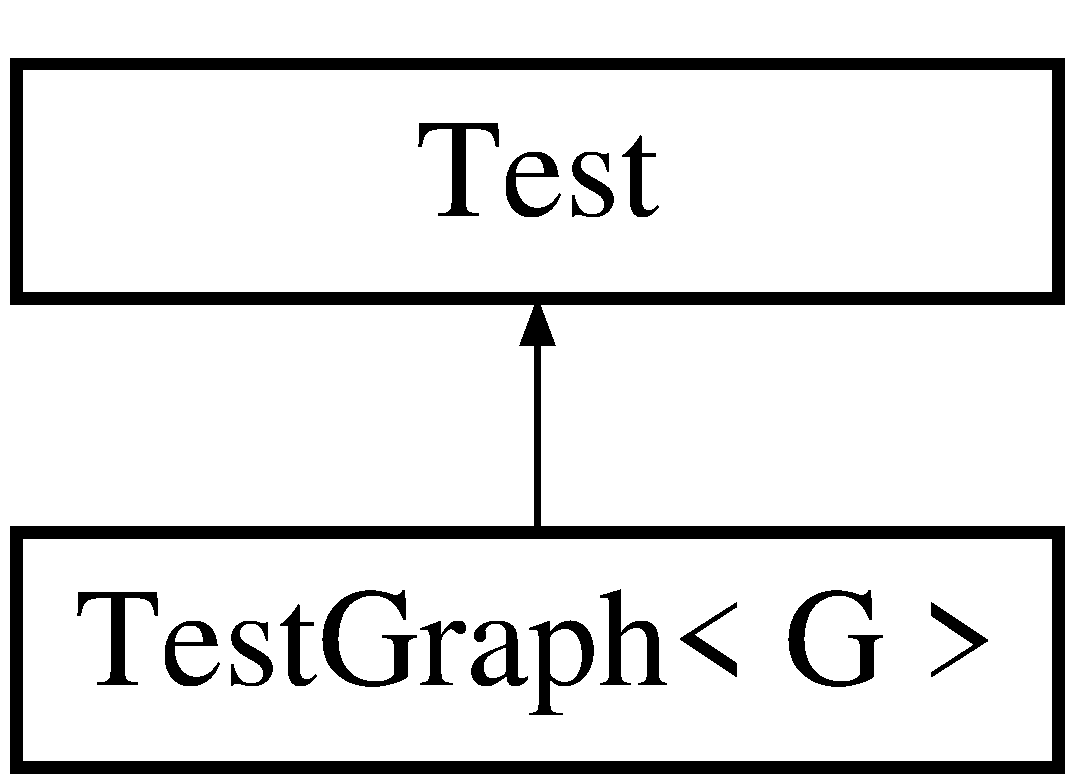
\includegraphics[height=2.000000cm]{structTestGraph}
\end{center}
\end{figure}
\subsection*{Public Types}
\begin{DoxyCompactItemize}
\item 
typedef G \hyperlink{structTestGraph_a149d9d185e2299b108590e2f83804351}{graph\-\_\-type}
\item 
typedef G\-::vertex\-\_\-descriptor \hyperlink{structTestGraph_aa82e61846643af7ce36a6993b81b9aa3}{vertex\-\_\-descriptor}
\item 
typedef G\-::edge\-\_\-descriptor \hyperlink{structTestGraph_aa20b87dd86a6d46d79cd5eead7e3ecd8}{edge\-\_\-descriptor}
\item 
typedef G\-::vertex\-\_\-iterator \hyperlink{structTestGraph_ae82be295babd001adfdf636fc39a79f8}{vertex\-\_\-iterator}
\item 
typedef G\-::edge\-\_\-iterator \hyperlink{structTestGraph_a4a62a3acea29caad985cde5504e4222d}{edge\-\_\-iterator}
\item 
typedef G\-::adjacency\-\_\-iterator \hyperlink{structTestGraph_af50caf6f726568b4165d4a1dc5b75cc3}{adjacency\-\_\-iterator}
\item 
typedef G\-::vertices\-\_\-size\-\_\-type \hyperlink{structTestGraph_a808d6ca09652f1c14f6a68ca42beb447}{vertices\-\_\-size\-\_\-type}
\item 
typedef G\-::edges\-\_\-size\-\_\-type \hyperlink{structTestGraph_a308c6aa7034bf56790d592b0fc259851}{edges\-\_\-size\-\_\-type}
\end{DoxyCompactItemize}


\subsection{Member Typedef Documentation}
\hypertarget{structTestGraph_af50caf6f726568b4165d4a1dc5b75cc3}{\index{Test\-Graph@{Test\-Graph}!adjacency\-\_\-iterator@{adjacency\-\_\-iterator}}
\index{adjacency\-\_\-iterator@{adjacency\-\_\-iterator}!TestGraph@{Test\-Graph}}
\subsubsection[{adjacency\-\_\-iterator}]{\setlength{\rightskip}{0pt plus 5cm}template$<$typename G $>$ typedef G\-::adjacency\-\_\-iterator {\bf Test\-Graph}$<$ G $>$\-::{\bf adjacency\-\_\-iterator}}}\label{structTestGraph_af50caf6f726568b4165d4a1dc5b75cc3}
\hypertarget{structTestGraph_aa20b87dd86a6d46d79cd5eead7e3ecd8}{\index{Test\-Graph@{Test\-Graph}!edge\-\_\-descriptor@{edge\-\_\-descriptor}}
\index{edge\-\_\-descriptor@{edge\-\_\-descriptor}!TestGraph@{Test\-Graph}}
\subsubsection[{edge\-\_\-descriptor}]{\setlength{\rightskip}{0pt plus 5cm}template$<$typename G $>$ typedef G\-::edge\-\_\-descriptor {\bf Test\-Graph}$<$ G $>$\-::{\bf edge\-\_\-descriptor}}}\label{structTestGraph_aa20b87dd86a6d46d79cd5eead7e3ecd8}
\hypertarget{structTestGraph_a4a62a3acea29caad985cde5504e4222d}{\index{Test\-Graph@{Test\-Graph}!edge\-\_\-iterator@{edge\-\_\-iterator}}
\index{edge\-\_\-iterator@{edge\-\_\-iterator}!TestGraph@{Test\-Graph}}
\subsubsection[{edge\-\_\-iterator}]{\setlength{\rightskip}{0pt plus 5cm}template$<$typename G $>$ typedef G\-::edge\-\_\-iterator {\bf Test\-Graph}$<$ G $>$\-::{\bf edge\-\_\-iterator}}}\label{structTestGraph_a4a62a3acea29caad985cde5504e4222d}
\hypertarget{structTestGraph_a308c6aa7034bf56790d592b0fc259851}{\index{Test\-Graph@{Test\-Graph}!edges\-\_\-size\-\_\-type@{edges\-\_\-size\-\_\-type}}
\index{edges\-\_\-size\-\_\-type@{edges\-\_\-size\-\_\-type}!TestGraph@{Test\-Graph}}
\subsubsection[{edges\-\_\-size\-\_\-type}]{\setlength{\rightskip}{0pt plus 5cm}template$<$typename G $>$ typedef G\-::edges\-\_\-size\-\_\-type {\bf Test\-Graph}$<$ G $>$\-::{\bf edges\-\_\-size\-\_\-type}}}\label{structTestGraph_a308c6aa7034bf56790d592b0fc259851}
\hypertarget{structTestGraph_a149d9d185e2299b108590e2f83804351}{\index{Test\-Graph@{Test\-Graph}!graph\-\_\-type@{graph\-\_\-type}}
\index{graph\-\_\-type@{graph\-\_\-type}!TestGraph@{Test\-Graph}}
\subsubsection[{graph\-\_\-type}]{\setlength{\rightskip}{0pt plus 5cm}template$<$typename G $>$ typedef G {\bf Test\-Graph}$<$ G $>$\-::{\bf graph\-\_\-type}}}\label{structTestGraph_a149d9d185e2299b108590e2f83804351}
\hypertarget{structTestGraph_aa82e61846643af7ce36a6993b81b9aa3}{\index{Test\-Graph@{Test\-Graph}!vertex\-\_\-descriptor@{vertex\-\_\-descriptor}}
\index{vertex\-\_\-descriptor@{vertex\-\_\-descriptor}!TestGraph@{Test\-Graph}}
\subsubsection[{vertex\-\_\-descriptor}]{\setlength{\rightskip}{0pt plus 5cm}template$<$typename G $>$ typedef G\-::vertex\-\_\-descriptor {\bf Test\-Graph}$<$ G $>$\-::{\bf vertex\-\_\-descriptor}}}\label{structTestGraph_aa82e61846643af7ce36a6993b81b9aa3}
\hypertarget{structTestGraph_ae82be295babd001adfdf636fc39a79f8}{\index{Test\-Graph@{Test\-Graph}!vertex\-\_\-iterator@{vertex\-\_\-iterator}}
\index{vertex\-\_\-iterator@{vertex\-\_\-iterator}!TestGraph@{Test\-Graph}}
\subsubsection[{vertex\-\_\-iterator}]{\setlength{\rightskip}{0pt plus 5cm}template$<$typename G $>$ typedef G\-::vertex\-\_\-iterator {\bf Test\-Graph}$<$ G $>$\-::{\bf vertex\-\_\-iterator}}}\label{structTestGraph_ae82be295babd001adfdf636fc39a79f8}
\hypertarget{structTestGraph_a808d6ca09652f1c14f6a68ca42beb447}{\index{Test\-Graph@{Test\-Graph}!vertices\-\_\-size\-\_\-type@{vertices\-\_\-size\-\_\-type}}
\index{vertices\-\_\-size\-\_\-type@{vertices\-\_\-size\-\_\-type}!TestGraph@{Test\-Graph}}
\subsubsection[{vertices\-\_\-size\-\_\-type}]{\setlength{\rightskip}{0pt plus 5cm}template$<$typename G $>$ typedef G\-::vertices\-\_\-size\-\_\-type {\bf Test\-Graph}$<$ G $>$\-::{\bf vertices\-\_\-size\-\_\-type}}}\label{structTestGraph_a808d6ca09652f1c14f6a68ca42beb447}


The documentation for this struct was generated from the following file\-:\begin{DoxyCompactItemize}
\item 
\hyperlink{TestGraph_8c_09_09}{Test\-Graph.\-c++}\end{DoxyCompactItemize}

\chapter{File Documentation}
\hypertarget{Graph_8h}{\section{Graph.\-h File Reference}
\label{Graph_8h}\index{Graph.\-h@{Graph.\-h}}
}
{\ttfamily \#include $<$cassert$>$}\\*
{\ttfamily \#include $<$cstddef$>$}\\*
{\ttfamily \#include $<$utility$>$}\\*
{\ttfamily \#include $<$vector$>$}\\*
\subsection*{Classes}
\begin{DoxyCompactItemize}
\item 
class \hyperlink{classGraph}{Graph}
\end{DoxyCompactItemize}

\hypertarget{TestGraph_8c_09_09}{\section{Test\-Graph.\-c++ File Reference}
\label{TestGraph_8c_09_09}\index{Test\-Graph.\-c++@{Test\-Graph.\-c++}}
}
{\ttfamily \#include $<$iostream$>$}\\*
{\ttfamily \#include $<$iterator$>$}\\*
{\ttfamily \#include $<$sstream$>$}\\*
{\ttfamily \#include $<$utility$>$}\\*
{\ttfamily \#include \char`\"{}boost/graph/adjacency\-\_\-list.\-hpp\char`\"{}}\\*
{\ttfamily \#include \char`\"{}boost/graph/topological\-\_\-sort.\-hpp\char`\"{}}\\*
{\ttfamily \#include \char`\"{}gtest/gtest.\-h\char`\"{}}\\*
{\ttfamily \#include \char`\"{}Graph.\-h\char`\"{}}\\*
\subsection*{Classes}
\begin{DoxyCompactItemize}
\item 
struct \hyperlink{structTestGraph}{Test\-Graph$<$ G $>$}
\end{DoxyCompactItemize}
\subsection*{Typedefs}
\begin{DoxyCompactItemize}
\item 
typedef Types\\*
$<$ boost\-::adjacency\-\_\-list\\*
$<$ boost\-::set\-S, boost\-::vec\-S, \\*
boost\-::directed\-S $>$, \hyperlink{classGraph}{Graph} $>$ \hyperlink{TestGraph_8c_09_09_ab8e2ae2a7026aca598606c55b1494184}{graph\-\_\-types}
\end{DoxyCompactItemize}
\subsection*{Functions}
\begin{DoxyCompactItemize}
\item 
\hyperlink{TestGraph_8c_09_09_a93499b72b807dd804b034251e923d425}{T\-Y\-P\-E\-D\-\_\-\-T\-E\-S\-T\-\_\-\-C\-A\-S\-E} (\hyperlink{structTestGraph}{Test\-Graph}, \hyperlink{TestGraph_8c_09_09_ab8e2ae2a7026aca598606c55b1494184}{graph\-\_\-types})
\item 
\hyperlink{TestGraph_8c_09_09_a846fbbada4644eb5ed8aad1d8c66ac1d}{T\-Y\-P\-E\-D\-\_\-\-T\-E\-S\-T} (\hyperlink{structTestGraph}{Test\-Graph}, add\-\_\-edge\-\_\-1)
\item 
\hyperlink{TestGraph_8c_09_09_ae6995b22e45418716483ede892d6409d}{T\-Y\-P\-E\-D\-\_\-\-T\-E\-S\-T} (\hyperlink{structTestGraph}{Test\-Graph}, add\-\_\-edge\-\_\-2)
\item 
\hyperlink{TestGraph_8c_09_09_adef122e25bb2d21a272bff56bd75ece3}{T\-Y\-P\-E\-D\-\_\-\-T\-E\-S\-T} (\hyperlink{structTestGraph}{Test\-Graph}, add\-\_\-edge\-\_\-3)
\item 
\hyperlink{TestGraph_8c_09_09_aa62185520e0cce0f3bcfecdac81f00f8}{T\-Y\-P\-E\-D\-\_\-\-T\-E\-S\-T} (\hyperlink{structTestGraph}{Test\-Graph}, add\-\_\-vertex\-\_\-1)
\item 
\hyperlink{TestGraph_8c_09_09_a5730ee3afd8d1a4036569b96b739eebe}{T\-Y\-P\-E\-D\-\_\-\-T\-E\-S\-T} (\hyperlink{structTestGraph}{Test\-Graph}, add\-\_\-vertex\-\_\-2)
\item 
\hyperlink{TestGraph_8c_09_09_a067dd8799211220c6fd63e53b63c6545}{T\-Y\-P\-E\-D\-\_\-\-T\-E\-S\-T} (\hyperlink{structTestGraph}{Test\-Graph}, add\-\_\-vertex\-\_\-3)
\item 
\hyperlink{TestGraph_8c_09_09_a4f145c2f2e3fe8f99d0ab9f6d16839c5}{T\-Y\-P\-E\-D\-\_\-\-T\-E\-S\-T} (\hyperlink{structTestGraph}{Test\-Graph}, adjacent\-\_\-vertices\-\_\-1)
\item 
\hyperlink{TestGraph_8c_09_09_a098fdd8ff786d99b9f1e8d8bbf48cb01}{T\-Y\-P\-E\-D\-\_\-\-T\-E\-S\-T} (\hyperlink{structTestGraph}{Test\-Graph}, adjacent\-\_\-vertices\-\_\-2)
\item 
\hyperlink{TestGraph_8c_09_09_a8a08b08a003dc2c400c7ed1202bc9c79}{T\-Y\-P\-E\-D\-\_\-\-T\-E\-S\-T} (\hyperlink{structTestGraph}{Test\-Graph}, adjacent\-\_\-vertices\-\_\-3)
\item 
\hyperlink{TestGraph_8c_09_09_a652498d7062532c4a8c78ed9c91b22f0}{T\-Y\-P\-E\-D\-\_\-\-T\-E\-S\-T} (\hyperlink{structTestGraph}{Test\-Graph}, edge\-\_\-1)
\item 
\hyperlink{TestGraph_8c_09_09_aad4343580eecd66e01fbfa72fc187be2}{T\-Y\-P\-E\-D\-\_\-\-T\-E\-S\-T} (\hyperlink{structTestGraph}{Test\-Graph}, edge\-\_\-2)
\item 
\hyperlink{TestGraph_8c_09_09_a90edf01026cf16dac993c6a6e140aaa3}{T\-Y\-P\-E\-D\-\_\-\-T\-E\-S\-T} (\hyperlink{structTestGraph}{Test\-Graph}, edge\-\_\-3)
\item 
\hyperlink{TestGraph_8c_09_09_a9493a0d1f567d7558cd314493729f970}{T\-Y\-P\-E\-D\-\_\-\-T\-E\-S\-T} (\hyperlink{structTestGraph}{Test\-Graph}, edges\-\_\-1)
\item 
\hyperlink{TestGraph_8c_09_09_af87ba0f65937bbe791cd293d33e396f6}{T\-Y\-P\-E\-D\-\_\-\-T\-E\-S\-T} (\hyperlink{structTestGraph}{Test\-Graph}, edges\-\_\-2)
\item 
\hyperlink{TestGraph_8c_09_09_a8826c3ba737abbf42008031e0f4ea825}{T\-Y\-P\-E\-D\-\_\-\-T\-E\-S\-T} (\hyperlink{structTestGraph}{Test\-Graph}, edges\-\_\-3)
\item 
\hyperlink{TestGraph_8c_09_09_ac4721f35b1c6b4abe5077658583699d1}{T\-Y\-P\-E\-D\-\_\-\-T\-E\-S\-T} (\hyperlink{structTestGraph}{Test\-Graph}, num\-\_\-edges\-\_\-1)
\item 
\hyperlink{TestGraph_8c_09_09_a10b5de405692802242cb86c40eeaa4dd}{T\-Y\-P\-E\-D\-\_\-\-T\-E\-S\-T} (\hyperlink{structTestGraph}{Test\-Graph}, num\-\_\-edges\-\_\-2)
\item 
\hyperlink{TestGraph_8c_09_09_a3f03d716c6d5ea85c635f45fd4b250a1}{T\-Y\-P\-E\-D\-\_\-\-T\-E\-S\-T} (\hyperlink{structTestGraph}{Test\-Graph}, num\-\_\-edges\-\_\-3)
\item 
\hyperlink{TestGraph_8c_09_09_a38ddfb80aeab11d5f9f96e301636dc8f}{T\-Y\-P\-E\-D\-\_\-\-T\-E\-S\-T} (\hyperlink{structTestGraph}{Test\-Graph}, num\-\_\-vertices\-\_\-1)
\item 
\hyperlink{TestGraph_8c_09_09_a45508ab23064846bef4aa8b665e1fc28}{T\-Y\-P\-E\-D\-\_\-\-T\-E\-S\-T} (\hyperlink{structTestGraph}{Test\-Graph}, num\-\_\-vertices\-\_\-2)
\item 
\hyperlink{TestGraph_8c_09_09_afd8bb41ac894f28c3e65a943fdda9058}{T\-Y\-P\-E\-D\-\_\-\-T\-E\-S\-T} (\hyperlink{structTestGraph}{Test\-Graph}, num\-\_\-vertices\-\_\-3)
\item 
\hyperlink{TestGraph_8c_09_09_ad5b455f84e90315d59d297f6683ba49c}{T\-Y\-P\-E\-D\-\_\-\-T\-E\-S\-T} (\hyperlink{structTestGraph}{Test\-Graph}, num\-\_\-vertices\-\_\-4)
\item 
\hyperlink{TestGraph_8c_09_09_a357f69e0c65ffe837c1a50cc9abf4446}{T\-Y\-P\-E\-D\-\_\-\-T\-E\-S\-T} (\hyperlink{structTestGraph}{Test\-Graph}, source\-\_\-1)
\item 
\hyperlink{TestGraph_8c_09_09_a7d3363f4d6c52571fadda44674aec77e}{T\-Y\-P\-E\-D\-\_\-\-T\-E\-S\-T} (\hyperlink{structTestGraph}{Test\-Graph}, source\-\_\-2)
\item 
\hyperlink{TestGraph_8c_09_09_aa5dcf214c2d72e66980984f8683d5f51}{T\-Y\-P\-E\-D\-\_\-\-T\-E\-S\-T} (\hyperlink{structTestGraph}{Test\-Graph}, source\-\_\-3)
\item 
\hyperlink{TestGraph_8c_09_09_a7ddc1d9ef8cc196aaad7d311559ff7d6}{T\-Y\-P\-E\-D\-\_\-\-T\-E\-S\-T} (\hyperlink{structTestGraph}{Test\-Graph}, target\-\_\-1)
\item 
\hyperlink{TestGraph_8c_09_09_aebbe5b19d3d08ea67d41407013c68730}{T\-Y\-P\-E\-D\-\_\-\-T\-E\-S\-T} (\hyperlink{structTestGraph}{Test\-Graph}, target\-\_\-2)
\item 
\hyperlink{TestGraph_8c_09_09_a70a2ce9b52f75a14f93d3578a5da6eb3}{T\-Y\-P\-E\-D\-\_\-\-T\-E\-S\-T} (\hyperlink{structTestGraph}{Test\-Graph}, target\-\_\-3)
\item 
\hyperlink{TestGraph_8c_09_09_a7d1dcfb2ea67c0d7f50542e69c6d2822}{T\-Y\-P\-E\-D\-\_\-\-T\-E\-S\-T} (\hyperlink{structTestGraph}{Test\-Graph}, vertex\-\_\-1)
\item 
\hyperlink{TestGraph_8c_09_09_a6332eae99dce8de9ea880f7765b9936d}{T\-Y\-P\-E\-D\-\_\-\-T\-E\-S\-T} (\hyperlink{structTestGraph}{Test\-Graph}, vertex\-\_\-2)
\item 
\hyperlink{TestGraph_8c_09_09_af1ebb553dde33bf2791f69dc0bc4fc18}{T\-Y\-P\-E\-D\-\_\-\-T\-E\-S\-T} (\hyperlink{structTestGraph}{Test\-Graph}, vertex\-\_\-3)
\item 
\hyperlink{TestGraph_8c_09_09_a2124e1f4ee8757af5339965a3334870b}{T\-Y\-P\-E\-D\-\_\-\-T\-E\-S\-T} (\hyperlink{structTestGraph}{Test\-Graph}, vertices\-\_\-1)
\item 
\hyperlink{TestGraph_8c_09_09_a427a2ce02293c7a4a6a737a909fb02ab}{T\-Y\-P\-E\-D\-\_\-\-T\-E\-S\-T} (\hyperlink{structTestGraph}{Test\-Graph}, vertices\-\_\-2)
\item 
\hyperlink{TestGraph_8c_09_09_a2f5f39f924c6da4fbcfea85cdefe748d}{T\-Y\-P\-E\-D\-\_\-\-T\-E\-S\-T} (\hyperlink{structTestGraph}{Test\-Graph}, vertices\-\_\-3)
\item 
\hyperlink{TestGraph_8c_09_09_a81fb7ad1df37e5d1fc4747bd056c971b}{T\-Y\-P\-E\-D\-\_\-\-T\-E\-S\-T} (\hyperlink{structTestGraph}{Test\-Graph}, constructor\-\_\-1)
\item 
\hyperlink{TestGraph_8c_09_09_a30c7f279598e0e14a1625ed11f655aad}{T\-Y\-P\-E\-D\-\_\-\-T\-E\-S\-T} (\hyperlink{structTestGraph}{Test\-Graph}, constructor\-\_\-2)
\item 
\hyperlink{TestGraph_8c_09_09_af3fff20b93f0116c698ff44507e76aa4}{T\-Y\-P\-E\-D\-\_\-\-T\-E\-S\-T} (\hyperlink{structTestGraph}{Test\-Graph}, test\-\_\-vertex)
\item 
\hyperlink{TestGraph_8c_09_09_a7a4ea6096b423811f225adb93948090c}{T\-Y\-P\-E\-D\-\_\-\-T\-E\-S\-T} (\hyperlink{structTestGraph}{Test\-Graph}, test\-\_\-edge)
\item 
\hyperlink{TestGraph_8c_09_09_a58a54238d1d9489afe62d6b3df215a2b}{T\-Y\-P\-E\-D\-\_\-\-T\-E\-S\-T} (\hyperlink{structTestGraph}{Test\-Graph}, test\-\_\-vertices)
\item 
\hyperlink{TestGraph_8c_09_09_a09a476a6046ae05f7120b420f6580b8a}{T\-Y\-P\-E\-D\-\_\-\-T\-E\-S\-T} (\hyperlink{structTestGraph}{Test\-Graph}, test\-\_\-edges)
\item 
\hyperlink{TestGraph_8c_09_09_a43218a1cef01d97a1961e19a18013334}{T\-Y\-P\-E\-D\-\_\-\-T\-E\-S\-T} (\hyperlink{structTestGraph}{Test\-Graph}, test\-\_\-adjacent\-\_\-vertices)
\end{DoxyCompactItemize}


\subsection{Typedef Documentation}
\hypertarget{TestGraph_8c_09_09_ab8e2ae2a7026aca598606c55b1494184}{\index{Test\-Graph.\-c++@{Test\-Graph.\-c++}!graph\-\_\-types@{graph\-\_\-types}}
\index{graph\-\_\-types@{graph\-\_\-types}!TestGraph.c++@{Test\-Graph.\-c++}}
\subsubsection[{graph\-\_\-types}]{\setlength{\rightskip}{0pt plus 5cm}typedef Types$<$ boost\-::adjacency\-\_\-list$<$boost\-::set\-S, boost\-::vec\-S, boost\-::directed\-S$>$, {\bf Graph}$>$ {\bf graph\-\_\-types}}}\label{TestGraph_8c_09_09_ab8e2ae2a7026aca598606c55b1494184}


\subsection{Function Documentation}
\hypertarget{TestGraph_8c_09_09_a846fbbada4644eb5ed8aad1d8c66ac1d}{\index{Test\-Graph.\-c++@{Test\-Graph.\-c++}!T\-Y\-P\-E\-D\-\_\-\-T\-E\-S\-T@{T\-Y\-P\-E\-D\-\_\-\-T\-E\-S\-T}}
\index{T\-Y\-P\-E\-D\-\_\-\-T\-E\-S\-T@{T\-Y\-P\-E\-D\-\_\-\-T\-E\-S\-T}!TestGraph.c++@{Test\-Graph.\-c++}}
\subsubsection[{T\-Y\-P\-E\-D\-\_\-\-T\-E\-S\-T}]{\setlength{\rightskip}{0pt plus 5cm}T\-Y\-P\-E\-D\-\_\-\-T\-E\-S\-T (
\begin{DoxyParamCaption}
\item[{{\bf Test\-Graph}}]{, }
\item[{add\-\_\-edge\-\_\-1}]{}
\end{DoxyParamCaption}
)}}\label{TestGraph_8c_09_09_a846fbbada4644eb5ed8aad1d8c66ac1d}
\hypertarget{TestGraph_8c_09_09_ae6995b22e45418716483ede892d6409d}{\index{Test\-Graph.\-c++@{Test\-Graph.\-c++}!T\-Y\-P\-E\-D\-\_\-\-T\-E\-S\-T@{T\-Y\-P\-E\-D\-\_\-\-T\-E\-S\-T}}
\index{T\-Y\-P\-E\-D\-\_\-\-T\-E\-S\-T@{T\-Y\-P\-E\-D\-\_\-\-T\-E\-S\-T}!TestGraph.c++@{Test\-Graph.\-c++}}
\subsubsection[{T\-Y\-P\-E\-D\-\_\-\-T\-E\-S\-T}]{\setlength{\rightskip}{0pt plus 5cm}T\-Y\-P\-E\-D\-\_\-\-T\-E\-S\-T (
\begin{DoxyParamCaption}
\item[{{\bf Test\-Graph}}]{, }
\item[{add\-\_\-edge\-\_\-2}]{}
\end{DoxyParamCaption}
)}}\label{TestGraph_8c_09_09_ae6995b22e45418716483ede892d6409d}
\hypertarget{TestGraph_8c_09_09_adef122e25bb2d21a272bff56bd75ece3}{\index{Test\-Graph.\-c++@{Test\-Graph.\-c++}!T\-Y\-P\-E\-D\-\_\-\-T\-E\-S\-T@{T\-Y\-P\-E\-D\-\_\-\-T\-E\-S\-T}}
\index{T\-Y\-P\-E\-D\-\_\-\-T\-E\-S\-T@{T\-Y\-P\-E\-D\-\_\-\-T\-E\-S\-T}!TestGraph.c++@{Test\-Graph.\-c++}}
\subsubsection[{T\-Y\-P\-E\-D\-\_\-\-T\-E\-S\-T}]{\setlength{\rightskip}{0pt plus 5cm}T\-Y\-P\-E\-D\-\_\-\-T\-E\-S\-T (
\begin{DoxyParamCaption}
\item[{{\bf Test\-Graph}}]{, }
\item[{add\-\_\-edge\-\_\-3}]{}
\end{DoxyParamCaption}
)}}\label{TestGraph_8c_09_09_adef122e25bb2d21a272bff56bd75ece3}
\hypertarget{TestGraph_8c_09_09_aa62185520e0cce0f3bcfecdac81f00f8}{\index{Test\-Graph.\-c++@{Test\-Graph.\-c++}!T\-Y\-P\-E\-D\-\_\-\-T\-E\-S\-T@{T\-Y\-P\-E\-D\-\_\-\-T\-E\-S\-T}}
\index{T\-Y\-P\-E\-D\-\_\-\-T\-E\-S\-T@{T\-Y\-P\-E\-D\-\_\-\-T\-E\-S\-T}!TestGraph.c++@{Test\-Graph.\-c++}}
\subsubsection[{T\-Y\-P\-E\-D\-\_\-\-T\-E\-S\-T}]{\setlength{\rightskip}{0pt plus 5cm}T\-Y\-P\-E\-D\-\_\-\-T\-E\-S\-T (
\begin{DoxyParamCaption}
\item[{{\bf Test\-Graph}}]{, }
\item[{add\-\_\-vertex\-\_\-1}]{}
\end{DoxyParamCaption}
)}}\label{TestGraph_8c_09_09_aa62185520e0cce0f3bcfecdac81f00f8}
\hypertarget{TestGraph_8c_09_09_a5730ee3afd8d1a4036569b96b739eebe}{\index{Test\-Graph.\-c++@{Test\-Graph.\-c++}!T\-Y\-P\-E\-D\-\_\-\-T\-E\-S\-T@{T\-Y\-P\-E\-D\-\_\-\-T\-E\-S\-T}}
\index{T\-Y\-P\-E\-D\-\_\-\-T\-E\-S\-T@{T\-Y\-P\-E\-D\-\_\-\-T\-E\-S\-T}!TestGraph.c++@{Test\-Graph.\-c++}}
\subsubsection[{T\-Y\-P\-E\-D\-\_\-\-T\-E\-S\-T}]{\setlength{\rightskip}{0pt plus 5cm}T\-Y\-P\-E\-D\-\_\-\-T\-E\-S\-T (
\begin{DoxyParamCaption}
\item[{{\bf Test\-Graph}}]{, }
\item[{add\-\_\-vertex\-\_\-2}]{}
\end{DoxyParamCaption}
)}}\label{TestGraph_8c_09_09_a5730ee3afd8d1a4036569b96b739eebe}
\hypertarget{TestGraph_8c_09_09_a067dd8799211220c6fd63e53b63c6545}{\index{Test\-Graph.\-c++@{Test\-Graph.\-c++}!T\-Y\-P\-E\-D\-\_\-\-T\-E\-S\-T@{T\-Y\-P\-E\-D\-\_\-\-T\-E\-S\-T}}
\index{T\-Y\-P\-E\-D\-\_\-\-T\-E\-S\-T@{T\-Y\-P\-E\-D\-\_\-\-T\-E\-S\-T}!TestGraph.c++@{Test\-Graph.\-c++}}
\subsubsection[{T\-Y\-P\-E\-D\-\_\-\-T\-E\-S\-T}]{\setlength{\rightskip}{0pt plus 5cm}T\-Y\-P\-E\-D\-\_\-\-T\-E\-S\-T (
\begin{DoxyParamCaption}
\item[{{\bf Test\-Graph}}]{, }
\item[{add\-\_\-vertex\-\_\-3}]{}
\end{DoxyParamCaption}
)}}\label{TestGraph_8c_09_09_a067dd8799211220c6fd63e53b63c6545}
\hypertarget{TestGraph_8c_09_09_a4f145c2f2e3fe8f99d0ab9f6d16839c5}{\index{Test\-Graph.\-c++@{Test\-Graph.\-c++}!T\-Y\-P\-E\-D\-\_\-\-T\-E\-S\-T@{T\-Y\-P\-E\-D\-\_\-\-T\-E\-S\-T}}
\index{T\-Y\-P\-E\-D\-\_\-\-T\-E\-S\-T@{T\-Y\-P\-E\-D\-\_\-\-T\-E\-S\-T}!TestGraph.c++@{Test\-Graph.\-c++}}
\subsubsection[{T\-Y\-P\-E\-D\-\_\-\-T\-E\-S\-T}]{\setlength{\rightskip}{0pt plus 5cm}T\-Y\-P\-E\-D\-\_\-\-T\-E\-S\-T (
\begin{DoxyParamCaption}
\item[{{\bf Test\-Graph}}]{, }
\item[{adjacent\-\_\-vertices\-\_\-1}]{}
\end{DoxyParamCaption}
)}}\label{TestGraph_8c_09_09_a4f145c2f2e3fe8f99d0ab9f6d16839c5}
\hypertarget{TestGraph_8c_09_09_a098fdd8ff786d99b9f1e8d8bbf48cb01}{\index{Test\-Graph.\-c++@{Test\-Graph.\-c++}!T\-Y\-P\-E\-D\-\_\-\-T\-E\-S\-T@{T\-Y\-P\-E\-D\-\_\-\-T\-E\-S\-T}}
\index{T\-Y\-P\-E\-D\-\_\-\-T\-E\-S\-T@{T\-Y\-P\-E\-D\-\_\-\-T\-E\-S\-T}!TestGraph.c++@{Test\-Graph.\-c++}}
\subsubsection[{T\-Y\-P\-E\-D\-\_\-\-T\-E\-S\-T}]{\setlength{\rightskip}{0pt plus 5cm}T\-Y\-P\-E\-D\-\_\-\-T\-E\-S\-T (
\begin{DoxyParamCaption}
\item[{{\bf Test\-Graph}}]{, }
\item[{adjacent\-\_\-vertices\-\_\-2}]{}
\end{DoxyParamCaption}
)}}\label{TestGraph_8c_09_09_a098fdd8ff786d99b9f1e8d8bbf48cb01}
\hypertarget{TestGraph_8c_09_09_a8a08b08a003dc2c400c7ed1202bc9c79}{\index{Test\-Graph.\-c++@{Test\-Graph.\-c++}!T\-Y\-P\-E\-D\-\_\-\-T\-E\-S\-T@{T\-Y\-P\-E\-D\-\_\-\-T\-E\-S\-T}}
\index{T\-Y\-P\-E\-D\-\_\-\-T\-E\-S\-T@{T\-Y\-P\-E\-D\-\_\-\-T\-E\-S\-T}!TestGraph.c++@{Test\-Graph.\-c++}}
\subsubsection[{T\-Y\-P\-E\-D\-\_\-\-T\-E\-S\-T}]{\setlength{\rightskip}{0pt plus 5cm}T\-Y\-P\-E\-D\-\_\-\-T\-E\-S\-T (
\begin{DoxyParamCaption}
\item[{{\bf Test\-Graph}}]{, }
\item[{adjacent\-\_\-vertices\-\_\-3}]{}
\end{DoxyParamCaption}
)}}\label{TestGraph_8c_09_09_a8a08b08a003dc2c400c7ed1202bc9c79}
\hypertarget{TestGraph_8c_09_09_a652498d7062532c4a8c78ed9c91b22f0}{\index{Test\-Graph.\-c++@{Test\-Graph.\-c++}!T\-Y\-P\-E\-D\-\_\-\-T\-E\-S\-T@{T\-Y\-P\-E\-D\-\_\-\-T\-E\-S\-T}}
\index{T\-Y\-P\-E\-D\-\_\-\-T\-E\-S\-T@{T\-Y\-P\-E\-D\-\_\-\-T\-E\-S\-T}!TestGraph.c++@{Test\-Graph.\-c++}}
\subsubsection[{T\-Y\-P\-E\-D\-\_\-\-T\-E\-S\-T}]{\setlength{\rightskip}{0pt plus 5cm}T\-Y\-P\-E\-D\-\_\-\-T\-E\-S\-T (
\begin{DoxyParamCaption}
\item[{{\bf Test\-Graph}}]{, }
\item[{edge\-\_\-1}]{}
\end{DoxyParamCaption}
)}}\label{TestGraph_8c_09_09_a652498d7062532c4a8c78ed9c91b22f0}
\hypertarget{TestGraph_8c_09_09_aad4343580eecd66e01fbfa72fc187be2}{\index{Test\-Graph.\-c++@{Test\-Graph.\-c++}!T\-Y\-P\-E\-D\-\_\-\-T\-E\-S\-T@{T\-Y\-P\-E\-D\-\_\-\-T\-E\-S\-T}}
\index{T\-Y\-P\-E\-D\-\_\-\-T\-E\-S\-T@{T\-Y\-P\-E\-D\-\_\-\-T\-E\-S\-T}!TestGraph.c++@{Test\-Graph.\-c++}}
\subsubsection[{T\-Y\-P\-E\-D\-\_\-\-T\-E\-S\-T}]{\setlength{\rightskip}{0pt plus 5cm}T\-Y\-P\-E\-D\-\_\-\-T\-E\-S\-T (
\begin{DoxyParamCaption}
\item[{{\bf Test\-Graph}}]{, }
\item[{edge\-\_\-2}]{}
\end{DoxyParamCaption}
)}}\label{TestGraph_8c_09_09_aad4343580eecd66e01fbfa72fc187be2}
\hypertarget{TestGraph_8c_09_09_a90edf01026cf16dac993c6a6e140aaa3}{\index{Test\-Graph.\-c++@{Test\-Graph.\-c++}!T\-Y\-P\-E\-D\-\_\-\-T\-E\-S\-T@{T\-Y\-P\-E\-D\-\_\-\-T\-E\-S\-T}}
\index{T\-Y\-P\-E\-D\-\_\-\-T\-E\-S\-T@{T\-Y\-P\-E\-D\-\_\-\-T\-E\-S\-T}!TestGraph.c++@{Test\-Graph.\-c++}}
\subsubsection[{T\-Y\-P\-E\-D\-\_\-\-T\-E\-S\-T}]{\setlength{\rightskip}{0pt plus 5cm}T\-Y\-P\-E\-D\-\_\-\-T\-E\-S\-T (
\begin{DoxyParamCaption}
\item[{{\bf Test\-Graph}}]{, }
\item[{edge\-\_\-3}]{}
\end{DoxyParamCaption}
)}}\label{TestGraph_8c_09_09_a90edf01026cf16dac993c6a6e140aaa3}
\hypertarget{TestGraph_8c_09_09_a9493a0d1f567d7558cd314493729f970}{\index{Test\-Graph.\-c++@{Test\-Graph.\-c++}!T\-Y\-P\-E\-D\-\_\-\-T\-E\-S\-T@{T\-Y\-P\-E\-D\-\_\-\-T\-E\-S\-T}}
\index{T\-Y\-P\-E\-D\-\_\-\-T\-E\-S\-T@{T\-Y\-P\-E\-D\-\_\-\-T\-E\-S\-T}!TestGraph.c++@{Test\-Graph.\-c++}}
\subsubsection[{T\-Y\-P\-E\-D\-\_\-\-T\-E\-S\-T}]{\setlength{\rightskip}{0pt plus 5cm}T\-Y\-P\-E\-D\-\_\-\-T\-E\-S\-T (
\begin{DoxyParamCaption}
\item[{{\bf Test\-Graph}}]{, }
\item[{edges\-\_\-1}]{}
\end{DoxyParamCaption}
)}}\label{TestGraph_8c_09_09_a9493a0d1f567d7558cd314493729f970}
\hypertarget{TestGraph_8c_09_09_af87ba0f65937bbe791cd293d33e396f6}{\index{Test\-Graph.\-c++@{Test\-Graph.\-c++}!T\-Y\-P\-E\-D\-\_\-\-T\-E\-S\-T@{T\-Y\-P\-E\-D\-\_\-\-T\-E\-S\-T}}
\index{T\-Y\-P\-E\-D\-\_\-\-T\-E\-S\-T@{T\-Y\-P\-E\-D\-\_\-\-T\-E\-S\-T}!TestGraph.c++@{Test\-Graph.\-c++}}
\subsubsection[{T\-Y\-P\-E\-D\-\_\-\-T\-E\-S\-T}]{\setlength{\rightskip}{0pt plus 5cm}T\-Y\-P\-E\-D\-\_\-\-T\-E\-S\-T (
\begin{DoxyParamCaption}
\item[{{\bf Test\-Graph}}]{, }
\item[{edges\-\_\-2}]{}
\end{DoxyParamCaption}
)}}\label{TestGraph_8c_09_09_af87ba0f65937bbe791cd293d33e396f6}
\hypertarget{TestGraph_8c_09_09_a8826c3ba737abbf42008031e0f4ea825}{\index{Test\-Graph.\-c++@{Test\-Graph.\-c++}!T\-Y\-P\-E\-D\-\_\-\-T\-E\-S\-T@{T\-Y\-P\-E\-D\-\_\-\-T\-E\-S\-T}}
\index{T\-Y\-P\-E\-D\-\_\-\-T\-E\-S\-T@{T\-Y\-P\-E\-D\-\_\-\-T\-E\-S\-T}!TestGraph.c++@{Test\-Graph.\-c++}}
\subsubsection[{T\-Y\-P\-E\-D\-\_\-\-T\-E\-S\-T}]{\setlength{\rightskip}{0pt plus 5cm}T\-Y\-P\-E\-D\-\_\-\-T\-E\-S\-T (
\begin{DoxyParamCaption}
\item[{{\bf Test\-Graph}}]{, }
\item[{edges\-\_\-3}]{}
\end{DoxyParamCaption}
)}}\label{TestGraph_8c_09_09_a8826c3ba737abbf42008031e0f4ea825}
\hypertarget{TestGraph_8c_09_09_ac4721f35b1c6b4abe5077658583699d1}{\index{Test\-Graph.\-c++@{Test\-Graph.\-c++}!T\-Y\-P\-E\-D\-\_\-\-T\-E\-S\-T@{T\-Y\-P\-E\-D\-\_\-\-T\-E\-S\-T}}
\index{T\-Y\-P\-E\-D\-\_\-\-T\-E\-S\-T@{T\-Y\-P\-E\-D\-\_\-\-T\-E\-S\-T}!TestGraph.c++@{Test\-Graph.\-c++}}
\subsubsection[{T\-Y\-P\-E\-D\-\_\-\-T\-E\-S\-T}]{\setlength{\rightskip}{0pt plus 5cm}T\-Y\-P\-E\-D\-\_\-\-T\-E\-S\-T (
\begin{DoxyParamCaption}
\item[{{\bf Test\-Graph}}]{, }
\item[{num\-\_\-edges\-\_\-1}]{}
\end{DoxyParamCaption}
)}}\label{TestGraph_8c_09_09_ac4721f35b1c6b4abe5077658583699d1}
\hypertarget{TestGraph_8c_09_09_a10b5de405692802242cb86c40eeaa4dd}{\index{Test\-Graph.\-c++@{Test\-Graph.\-c++}!T\-Y\-P\-E\-D\-\_\-\-T\-E\-S\-T@{T\-Y\-P\-E\-D\-\_\-\-T\-E\-S\-T}}
\index{T\-Y\-P\-E\-D\-\_\-\-T\-E\-S\-T@{T\-Y\-P\-E\-D\-\_\-\-T\-E\-S\-T}!TestGraph.c++@{Test\-Graph.\-c++}}
\subsubsection[{T\-Y\-P\-E\-D\-\_\-\-T\-E\-S\-T}]{\setlength{\rightskip}{0pt plus 5cm}T\-Y\-P\-E\-D\-\_\-\-T\-E\-S\-T (
\begin{DoxyParamCaption}
\item[{{\bf Test\-Graph}}]{, }
\item[{num\-\_\-edges\-\_\-2}]{}
\end{DoxyParamCaption}
)}}\label{TestGraph_8c_09_09_a10b5de405692802242cb86c40eeaa4dd}
\hypertarget{TestGraph_8c_09_09_a3f03d716c6d5ea85c635f45fd4b250a1}{\index{Test\-Graph.\-c++@{Test\-Graph.\-c++}!T\-Y\-P\-E\-D\-\_\-\-T\-E\-S\-T@{T\-Y\-P\-E\-D\-\_\-\-T\-E\-S\-T}}
\index{T\-Y\-P\-E\-D\-\_\-\-T\-E\-S\-T@{T\-Y\-P\-E\-D\-\_\-\-T\-E\-S\-T}!TestGraph.c++@{Test\-Graph.\-c++}}
\subsubsection[{T\-Y\-P\-E\-D\-\_\-\-T\-E\-S\-T}]{\setlength{\rightskip}{0pt plus 5cm}T\-Y\-P\-E\-D\-\_\-\-T\-E\-S\-T (
\begin{DoxyParamCaption}
\item[{{\bf Test\-Graph}}]{, }
\item[{num\-\_\-edges\-\_\-3}]{}
\end{DoxyParamCaption}
)}}\label{TestGraph_8c_09_09_a3f03d716c6d5ea85c635f45fd4b250a1}
\hypertarget{TestGraph_8c_09_09_a38ddfb80aeab11d5f9f96e301636dc8f}{\index{Test\-Graph.\-c++@{Test\-Graph.\-c++}!T\-Y\-P\-E\-D\-\_\-\-T\-E\-S\-T@{T\-Y\-P\-E\-D\-\_\-\-T\-E\-S\-T}}
\index{T\-Y\-P\-E\-D\-\_\-\-T\-E\-S\-T@{T\-Y\-P\-E\-D\-\_\-\-T\-E\-S\-T}!TestGraph.c++@{Test\-Graph.\-c++}}
\subsubsection[{T\-Y\-P\-E\-D\-\_\-\-T\-E\-S\-T}]{\setlength{\rightskip}{0pt plus 5cm}T\-Y\-P\-E\-D\-\_\-\-T\-E\-S\-T (
\begin{DoxyParamCaption}
\item[{{\bf Test\-Graph}}]{, }
\item[{num\-\_\-vertices\-\_\-1}]{}
\end{DoxyParamCaption}
)}}\label{TestGraph_8c_09_09_a38ddfb80aeab11d5f9f96e301636dc8f}
\hypertarget{TestGraph_8c_09_09_a45508ab23064846bef4aa8b665e1fc28}{\index{Test\-Graph.\-c++@{Test\-Graph.\-c++}!T\-Y\-P\-E\-D\-\_\-\-T\-E\-S\-T@{T\-Y\-P\-E\-D\-\_\-\-T\-E\-S\-T}}
\index{T\-Y\-P\-E\-D\-\_\-\-T\-E\-S\-T@{T\-Y\-P\-E\-D\-\_\-\-T\-E\-S\-T}!TestGraph.c++@{Test\-Graph.\-c++}}
\subsubsection[{T\-Y\-P\-E\-D\-\_\-\-T\-E\-S\-T}]{\setlength{\rightskip}{0pt plus 5cm}T\-Y\-P\-E\-D\-\_\-\-T\-E\-S\-T (
\begin{DoxyParamCaption}
\item[{{\bf Test\-Graph}}]{, }
\item[{num\-\_\-vertices\-\_\-2}]{}
\end{DoxyParamCaption}
)}}\label{TestGraph_8c_09_09_a45508ab23064846bef4aa8b665e1fc28}
\hypertarget{TestGraph_8c_09_09_afd8bb41ac894f28c3e65a943fdda9058}{\index{Test\-Graph.\-c++@{Test\-Graph.\-c++}!T\-Y\-P\-E\-D\-\_\-\-T\-E\-S\-T@{T\-Y\-P\-E\-D\-\_\-\-T\-E\-S\-T}}
\index{T\-Y\-P\-E\-D\-\_\-\-T\-E\-S\-T@{T\-Y\-P\-E\-D\-\_\-\-T\-E\-S\-T}!TestGraph.c++@{Test\-Graph.\-c++}}
\subsubsection[{T\-Y\-P\-E\-D\-\_\-\-T\-E\-S\-T}]{\setlength{\rightskip}{0pt plus 5cm}T\-Y\-P\-E\-D\-\_\-\-T\-E\-S\-T (
\begin{DoxyParamCaption}
\item[{{\bf Test\-Graph}}]{, }
\item[{num\-\_\-vertices\-\_\-3}]{}
\end{DoxyParamCaption}
)}}\label{TestGraph_8c_09_09_afd8bb41ac894f28c3e65a943fdda9058}
\hypertarget{TestGraph_8c_09_09_ad5b455f84e90315d59d297f6683ba49c}{\index{Test\-Graph.\-c++@{Test\-Graph.\-c++}!T\-Y\-P\-E\-D\-\_\-\-T\-E\-S\-T@{T\-Y\-P\-E\-D\-\_\-\-T\-E\-S\-T}}
\index{T\-Y\-P\-E\-D\-\_\-\-T\-E\-S\-T@{T\-Y\-P\-E\-D\-\_\-\-T\-E\-S\-T}!TestGraph.c++@{Test\-Graph.\-c++}}
\subsubsection[{T\-Y\-P\-E\-D\-\_\-\-T\-E\-S\-T}]{\setlength{\rightskip}{0pt plus 5cm}T\-Y\-P\-E\-D\-\_\-\-T\-E\-S\-T (
\begin{DoxyParamCaption}
\item[{{\bf Test\-Graph}}]{, }
\item[{num\-\_\-vertices\-\_\-4}]{}
\end{DoxyParamCaption}
)}}\label{TestGraph_8c_09_09_ad5b455f84e90315d59d297f6683ba49c}
\hypertarget{TestGraph_8c_09_09_a357f69e0c65ffe837c1a50cc9abf4446}{\index{Test\-Graph.\-c++@{Test\-Graph.\-c++}!T\-Y\-P\-E\-D\-\_\-\-T\-E\-S\-T@{T\-Y\-P\-E\-D\-\_\-\-T\-E\-S\-T}}
\index{T\-Y\-P\-E\-D\-\_\-\-T\-E\-S\-T@{T\-Y\-P\-E\-D\-\_\-\-T\-E\-S\-T}!TestGraph.c++@{Test\-Graph.\-c++}}
\subsubsection[{T\-Y\-P\-E\-D\-\_\-\-T\-E\-S\-T}]{\setlength{\rightskip}{0pt plus 5cm}T\-Y\-P\-E\-D\-\_\-\-T\-E\-S\-T (
\begin{DoxyParamCaption}
\item[{{\bf Test\-Graph}}]{, }
\item[{source\-\_\-1}]{}
\end{DoxyParamCaption}
)}}\label{TestGraph_8c_09_09_a357f69e0c65ffe837c1a50cc9abf4446}
\hypertarget{TestGraph_8c_09_09_a7d3363f4d6c52571fadda44674aec77e}{\index{Test\-Graph.\-c++@{Test\-Graph.\-c++}!T\-Y\-P\-E\-D\-\_\-\-T\-E\-S\-T@{T\-Y\-P\-E\-D\-\_\-\-T\-E\-S\-T}}
\index{T\-Y\-P\-E\-D\-\_\-\-T\-E\-S\-T@{T\-Y\-P\-E\-D\-\_\-\-T\-E\-S\-T}!TestGraph.c++@{Test\-Graph.\-c++}}
\subsubsection[{T\-Y\-P\-E\-D\-\_\-\-T\-E\-S\-T}]{\setlength{\rightskip}{0pt plus 5cm}T\-Y\-P\-E\-D\-\_\-\-T\-E\-S\-T (
\begin{DoxyParamCaption}
\item[{{\bf Test\-Graph}}]{, }
\item[{source\-\_\-2}]{}
\end{DoxyParamCaption}
)}}\label{TestGraph_8c_09_09_a7d3363f4d6c52571fadda44674aec77e}
\hypertarget{TestGraph_8c_09_09_aa5dcf214c2d72e66980984f8683d5f51}{\index{Test\-Graph.\-c++@{Test\-Graph.\-c++}!T\-Y\-P\-E\-D\-\_\-\-T\-E\-S\-T@{T\-Y\-P\-E\-D\-\_\-\-T\-E\-S\-T}}
\index{T\-Y\-P\-E\-D\-\_\-\-T\-E\-S\-T@{T\-Y\-P\-E\-D\-\_\-\-T\-E\-S\-T}!TestGraph.c++@{Test\-Graph.\-c++}}
\subsubsection[{T\-Y\-P\-E\-D\-\_\-\-T\-E\-S\-T}]{\setlength{\rightskip}{0pt plus 5cm}T\-Y\-P\-E\-D\-\_\-\-T\-E\-S\-T (
\begin{DoxyParamCaption}
\item[{{\bf Test\-Graph}}]{, }
\item[{source\-\_\-3}]{}
\end{DoxyParamCaption}
)}}\label{TestGraph_8c_09_09_aa5dcf214c2d72e66980984f8683d5f51}
\hypertarget{TestGraph_8c_09_09_a7ddc1d9ef8cc196aaad7d311559ff7d6}{\index{Test\-Graph.\-c++@{Test\-Graph.\-c++}!T\-Y\-P\-E\-D\-\_\-\-T\-E\-S\-T@{T\-Y\-P\-E\-D\-\_\-\-T\-E\-S\-T}}
\index{T\-Y\-P\-E\-D\-\_\-\-T\-E\-S\-T@{T\-Y\-P\-E\-D\-\_\-\-T\-E\-S\-T}!TestGraph.c++@{Test\-Graph.\-c++}}
\subsubsection[{T\-Y\-P\-E\-D\-\_\-\-T\-E\-S\-T}]{\setlength{\rightskip}{0pt plus 5cm}T\-Y\-P\-E\-D\-\_\-\-T\-E\-S\-T (
\begin{DoxyParamCaption}
\item[{{\bf Test\-Graph}}]{, }
\item[{target\-\_\-1}]{}
\end{DoxyParamCaption}
)}}\label{TestGraph_8c_09_09_a7ddc1d9ef8cc196aaad7d311559ff7d6}
\hypertarget{TestGraph_8c_09_09_aebbe5b19d3d08ea67d41407013c68730}{\index{Test\-Graph.\-c++@{Test\-Graph.\-c++}!T\-Y\-P\-E\-D\-\_\-\-T\-E\-S\-T@{T\-Y\-P\-E\-D\-\_\-\-T\-E\-S\-T}}
\index{T\-Y\-P\-E\-D\-\_\-\-T\-E\-S\-T@{T\-Y\-P\-E\-D\-\_\-\-T\-E\-S\-T}!TestGraph.c++@{Test\-Graph.\-c++}}
\subsubsection[{T\-Y\-P\-E\-D\-\_\-\-T\-E\-S\-T}]{\setlength{\rightskip}{0pt plus 5cm}T\-Y\-P\-E\-D\-\_\-\-T\-E\-S\-T (
\begin{DoxyParamCaption}
\item[{{\bf Test\-Graph}}]{, }
\item[{target\-\_\-2}]{}
\end{DoxyParamCaption}
)}}\label{TestGraph_8c_09_09_aebbe5b19d3d08ea67d41407013c68730}
\hypertarget{TestGraph_8c_09_09_a70a2ce9b52f75a14f93d3578a5da6eb3}{\index{Test\-Graph.\-c++@{Test\-Graph.\-c++}!T\-Y\-P\-E\-D\-\_\-\-T\-E\-S\-T@{T\-Y\-P\-E\-D\-\_\-\-T\-E\-S\-T}}
\index{T\-Y\-P\-E\-D\-\_\-\-T\-E\-S\-T@{T\-Y\-P\-E\-D\-\_\-\-T\-E\-S\-T}!TestGraph.c++@{Test\-Graph.\-c++}}
\subsubsection[{T\-Y\-P\-E\-D\-\_\-\-T\-E\-S\-T}]{\setlength{\rightskip}{0pt plus 5cm}T\-Y\-P\-E\-D\-\_\-\-T\-E\-S\-T (
\begin{DoxyParamCaption}
\item[{{\bf Test\-Graph}}]{, }
\item[{target\-\_\-3}]{}
\end{DoxyParamCaption}
)}}\label{TestGraph_8c_09_09_a70a2ce9b52f75a14f93d3578a5da6eb3}
\hypertarget{TestGraph_8c_09_09_a7d1dcfb2ea67c0d7f50542e69c6d2822}{\index{Test\-Graph.\-c++@{Test\-Graph.\-c++}!T\-Y\-P\-E\-D\-\_\-\-T\-E\-S\-T@{T\-Y\-P\-E\-D\-\_\-\-T\-E\-S\-T}}
\index{T\-Y\-P\-E\-D\-\_\-\-T\-E\-S\-T@{T\-Y\-P\-E\-D\-\_\-\-T\-E\-S\-T}!TestGraph.c++@{Test\-Graph.\-c++}}
\subsubsection[{T\-Y\-P\-E\-D\-\_\-\-T\-E\-S\-T}]{\setlength{\rightskip}{0pt plus 5cm}T\-Y\-P\-E\-D\-\_\-\-T\-E\-S\-T (
\begin{DoxyParamCaption}
\item[{{\bf Test\-Graph}}]{, }
\item[{vertex\-\_\-1}]{}
\end{DoxyParamCaption}
)}}\label{TestGraph_8c_09_09_a7d1dcfb2ea67c0d7f50542e69c6d2822}
\hypertarget{TestGraph_8c_09_09_a6332eae99dce8de9ea880f7765b9936d}{\index{Test\-Graph.\-c++@{Test\-Graph.\-c++}!T\-Y\-P\-E\-D\-\_\-\-T\-E\-S\-T@{T\-Y\-P\-E\-D\-\_\-\-T\-E\-S\-T}}
\index{T\-Y\-P\-E\-D\-\_\-\-T\-E\-S\-T@{T\-Y\-P\-E\-D\-\_\-\-T\-E\-S\-T}!TestGraph.c++@{Test\-Graph.\-c++}}
\subsubsection[{T\-Y\-P\-E\-D\-\_\-\-T\-E\-S\-T}]{\setlength{\rightskip}{0pt plus 5cm}T\-Y\-P\-E\-D\-\_\-\-T\-E\-S\-T (
\begin{DoxyParamCaption}
\item[{{\bf Test\-Graph}}]{, }
\item[{vertex\-\_\-2}]{}
\end{DoxyParamCaption}
)}}\label{TestGraph_8c_09_09_a6332eae99dce8de9ea880f7765b9936d}
\hypertarget{TestGraph_8c_09_09_af1ebb553dde33bf2791f69dc0bc4fc18}{\index{Test\-Graph.\-c++@{Test\-Graph.\-c++}!T\-Y\-P\-E\-D\-\_\-\-T\-E\-S\-T@{T\-Y\-P\-E\-D\-\_\-\-T\-E\-S\-T}}
\index{T\-Y\-P\-E\-D\-\_\-\-T\-E\-S\-T@{T\-Y\-P\-E\-D\-\_\-\-T\-E\-S\-T}!TestGraph.c++@{Test\-Graph.\-c++}}
\subsubsection[{T\-Y\-P\-E\-D\-\_\-\-T\-E\-S\-T}]{\setlength{\rightskip}{0pt plus 5cm}T\-Y\-P\-E\-D\-\_\-\-T\-E\-S\-T (
\begin{DoxyParamCaption}
\item[{{\bf Test\-Graph}}]{, }
\item[{vertex\-\_\-3}]{}
\end{DoxyParamCaption}
)}}\label{TestGraph_8c_09_09_af1ebb553dde33bf2791f69dc0bc4fc18}
\hypertarget{TestGraph_8c_09_09_a2124e1f4ee8757af5339965a3334870b}{\index{Test\-Graph.\-c++@{Test\-Graph.\-c++}!T\-Y\-P\-E\-D\-\_\-\-T\-E\-S\-T@{T\-Y\-P\-E\-D\-\_\-\-T\-E\-S\-T}}
\index{T\-Y\-P\-E\-D\-\_\-\-T\-E\-S\-T@{T\-Y\-P\-E\-D\-\_\-\-T\-E\-S\-T}!TestGraph.c++@{Test\-Graph.\-c++}}
\subsubsection[{T\-Y\-P\-E\-D\-\_\-\-T\-E\-S\-T}]{\setlength{\rightskip}{0pt plus 5cm}T\-Y\-P\-E\-D\-\_\-\-T\-E\-S\-T (
\begin{DoxyParamCaption}
\item[{{\bf Test\-Graph}}]{, }
\item[{vertices\-\_\-1}]{}
\end{DoxyParamCaption}
)}}\label{TestGraph_8c_09_09_a2124e1f4ee8757af5339965a3334870b}
\hypertarget{TestGraph_8c_09_09_a427a2ce02293c7a4a6a737a909fb02ab}{\index{Test\-Graph.\-c++@{Test\-Graph.\-c++}!T\-Y\-P\-E\-D\-\_\-\-T\-E\-S\-T@{T\-Y\-P\-E\-D\-\_\-\-T\-E\-S\-T}}
\index{T\-Y\-P\-E\-D\-\_\-\-T\-E\-S\-T@{T\-Y\-P\-E\-D\-\_\-\-T\-E\-S\-T}!TestGraph.c++@{Test\-Graph.\-c++}}
\subsubsection[{T\-Y\-P\-E\-D\-\_\-\-T\-E\-S\-T}]{\setlength{\rightskip}{0pt plus 5cm}T\-Y\-P\-E\-D\-\_\-\-T\-E\-S\-T (
\begin{DoxyParamCaption}
\item[{{\bf Test\-Graph}}]{, }
\item[{vertices\-\_\-2}]{}
\end{DoxyParamCaption}
)}}\label{TestGraph_8c_09_09_a427a2ce02293c7a4a6a737a909fb02ab}
\hypertarget{TestGraph_8c_09_09_a2f5f39f924c6da4fbcfea85cdefe748d}{\index{Test\-Graph.\-c++@{Test\-Graph.\-c++}!T\-Y\-P\-E\-D\-\_\-\-T\-E\-S\-T@{T\-Y\-P\-E\-D\-\_\-\-T\-E\-S\-T}}
\index{T\-Y\-P\-E\-D\-\_\-\-T\-E\-S\-T@{T\-Y\-P\-E\-D\-\_\-\-T\-E\-S\-T}!TestGraph.c++@{Test\-Graph.\-c++}}
\subsubsection[{T\-Y\-P\-E\-D\-\_\-\-T\-E\-S\-T}]{\setlength{\rightskip}{0pt plus 5cm}T\-Y\-P\-E\-D\-\_\-\-T\-E\-S\-T (
\begin{DoxyParamCaption}
\item[{{\bf Test\-Graph}}]{, }
\item[{vertices\-\_\-3}]{}
\end{DoxyParamCaption}
)}}\label{TestGraph_8c_09_09_a2f5f39f924c6da4fbcfea85cdefe748d}
\hypertarget{TestGraph_8c_09_09_a81fb7ad1df37e5d1fc4747bd056c971b}{\index{Test\-Graph.\-c++@{Test\-Graph.\-c++}!T\-Y\-P\-E\-D\-\_\-\-T\-E\-S\-T@{T\-Y\-P\-E\-D\-\_\-\-T\-E\-S\-T}}
\index{T\-Y\-P\-E\-D\-\_\-\-T\-E\-S\-T@{T\-Y\-P\-E\-D\-\_\-\-T\-E\-S\-T}!TestGraph.c++@{Test\-Graph.\-c++}}
\subsubsection[{T\-Y\-P\-E\-D\-\_\-\-T\-E\-S\-T}]{\setlength{\rightskip}{0pt plus 5cm}T\-Y\-P\-E\-D\-\_\-\-T\-E\-S\-T (
\begin{DoxyParamCaption}
\item[{{\bf Test\-Graph}}]{, }
\item[{constructor\-\_\-1}]{}
\end{DoxyParamCaption}
)}}\label{TestGraph_8c_09_09_a81fb7ad1df37e5d1fc4747bd056c971b}
\hypertarget{TestGraph_8c_09_09_a30c7f279598e0e14a1625ed11f655aad}{\index{Test\-Graph.\-c++@{Test\-Graph.\-c++}!T\-Y\-P\-E\-D\-\_\-\-T\-E\-S\-T@{T\-Y\-P\-E\-D\-\_\-\-T\-E\-S\-T}}
\index{T\-Y\-P\-E\-D\-\_\-\-T\-E\-S\-T@{T\-Y\-P\-E\-D\-\_\-\-T\-E\-S\-T}!TestGraph.c++@{Test\-Graph.\-c++}}
\subsubsection[{T\-Y\-P\-E\-D\-\_\-\-T\-E\-S\-T}]{\setlength{\rightskip}{0pt plus 5cm}T\-Y\-P\-E\-D\-\_\-\-T\-E\-S\-T (
\begin{DoxyParamCaption}
\item[{{\bf Test\-Graph}}]{, }
\item[{constructor\-\_\-2}]{}
\end{DoxyParamCaption}
)}}\label{TestGraph_8c_09_09_a30c7f279598e0e14a1625ed11f655aad}
\hypertarget{TestGraph_8c_09_09_af3fff20b93f0116c698ff44507e76aa4}{\index{Test\-Graph.\-c++@{Test\-Graph.\-c++}!T\-Y\-P\-E\-D\-\_\-\-T\-E\-S\-T@{T\-Y\-P\-E\-D\-\_\-\-T\-E\-S\-T}}
\index{T\-Y\-P\-E\-D\-\_\-\-T\-E\-S\-T@{T\-Y\-P\-E\-D\-\_\-\-T\-E\-S\-T}!TestGraph.c++@{Test\-Graph.\-c++}}
\subsubsection[{T\-Y\-P\-E\-D\-\_\-\-T\-E\-S\-T}]{\setlength{\rightskip}{0pt plus 5cm}T\-Y\-P\-E\-D\-\_\-\-T\-E\-S\-T (
\begin{DoxyParamCaption}
\item[{{\bf Test\-Graph}}]{, }
\item[{test\-\_\-vertex}]{}
\end{DoxyParamCaption}
)}}\label{TestGraph_8c_09_09_af3fff20b93f0116c698ff44507e76aa4}
\hypertarget{TestGraph_8c_09_09_a7a4ea6096b423811f225adb93948090c}{\index{Test\-Graph.\-c++@{Test\-Graph.\-c++}!T\-Y\-P\-E\-D\-\_\-\-T\-E\-S\-T@{T\-Y\-P\-E\-D\-\_\-\-T\-E\-S\-T}}
\index{T\-Y\-P\-E\-D\-\_\-\-T\-E\-S\-T@{T\-Y\-P\-E\-D\-\_\-\-T\-E\-S\-T}!TestGraph.c++@{Test\-Graph.\-c++}}
\subsubsection[{T\-Y\-P\-E\-D\-\_\-\-T\-E\-S\-T}]{\setlength{\rightskip}{0pt plus 5cm}T\-Y\-P\-E\-D\-\_\-\-T\-E\-S\-T (
\begin{DoxyParamCaption}
\item[{{\bf Test\-Graph}}]{, }
\item[{test\-\_\-edge}]{}
\end{DoxyParamCaption}
)}}\label{TestGraph_8c_09_09_a7a4ea6096b423811f225adb93948090c}
\hypertarget{TestGraph_8c_09_09_a58a54238d1d9489afe62d6b3df215a2b}{\index{Test\-Graph.\-c++@{Test\-Graph.\-c++}!T\-Y\-P\-E\-D\-\_\-\-T\-E\-S\-T@{T\-Y\-P\-E\-D\-\_\-\-T\-E\-S\-T}}
\index{T\-Y\-P\-E\-D\-\_\-\-T\-E\-S\-T@{T\-Y\-P\-E\-D\-\_\-\-T\-E\-S\-T}!TestGraph.c++@{Test\-Graph.\-c++}}
\subsubsection[{T\-Y\-P\-E\-D\-\_\-\-T\-E\-S\-T}]{\setlength{\rightskip}{0pt plus 5cm}T\-Y\-P\-E\-D\-\_\-\-T\-E\-S\-T (
\begin{DoxyParamCaption}
\item[{{\bf Test\-Graph}}]{, }
\item[{test\-\_\-vertices}]{}
\end{DoxyParamCaption}
)}}\label{TestGraph_8c_09_09_a58a54238d1d9489afe62d6b3df215a2b}
\hypertarget{TestGraph_8c_09_09_a09a476a6046ae05f7120b420f6580b8a}{\index{Test\-Graph.\-c++@{Test\-Graph.\-c++}!T\-Y\-P\-E\-D\-\_\-\-T\-E\-S\-T@{T\-Y\-P\-E\-D\-\_\-\-T\-E\-S\-T}}
\index{T\-Y\-P\-E\-D\-\_\-\-T\-E\-S\-T@{T\-Y\-P\-E\-D\-\_\-\-T\-E\-S\-T}!TestGraph.c++@{Test\-Graph.\-c++}}
\subsubsection[{T\-Y\-P\-E\-D\-\_\-\-T\-E\-S\-T}]{\setlength{\rightskip}{0pt plus 5cm}T\-Y\-P\-E\-D\-\_\-\-T\-E\-S\-T (
\begin{DoxyParamCaption}
\item[{{\bf Test\-Graph}}]{, }
\item[{test\-\_\-edges}]{}
\end{DoxyParamCaption}
)}}\label{TestGraph_8c_09_09_a09a476a6046ae05f7120b420f6580b8a}
\hypertarget{TestGraph_8c_09_09_a43218a1cef01d97a1961e19a18013334}{\index{Test\-Graph.\-c++@{Test\-Graph.\-c++}!T\-Y\-P\-E\-D\-\_\-\-T\-E\-S\-T@{T\-Y\-P\-E\-D\-\_\-\-T\-E\-S\-T}}
\index{T\-Y\-P\-E\-D\-\_\-\-T\-E\-S\-T@{T\-Y\-P\-E\-D\-\_\-\-T\-E\-S\-T}!TestGraph.c++@{Test\-Graph.\-c++}}
\subsubsection[{T\-Y\-P\-E\-D\-\_\-\-T\-E\-S\-T}]{\setlength{\rightskip}{0pt plus 5cm}T\-Y\-P\-E\-D\-\_\-\-T\-E\-S\-T (
\begin{DoxyParamCaption}
\item[{{\bf Test\-Graph}}]{, }
\item[{test\-\_\-adjacent\-\_\-vertices}]{}
\end{DoxyParamCaption}
)}}\label{TestGraph_8c_09_09_a43218a1cef01d97a1961e19a18013334}
\hypertarget{TestGraph_8c_09_09_a93499b72b807dd804b034251e923d425}{\index{Test\-Graph.\-c++@{Test\-Graph.\-c++}!T\-Y\-P\-E\-D\-\_\-\-T\-E\-S\-T\-\_\-\-C\-A\-S\-E@{T\-Y\-P\-E\-D\-\_\-\-T\-E\-S\-T\-\_\-\-C\-A\-S\-E}}
\index{T\-Y\-P\-E\-D\-\_\-\-T\-E\-S\-T\-\_\-\-C\-A\-S\-E@{T\-Y\-P\-E\-D\-\_\-\-T\-E\-S\-T\-\_\-\-C\-A\-S\-E}!TestGraph.c++@{Test\-Graph.\-c++}}
\subsubsection[{T\-Y\-P\-E\-D\-\_\-\-T\-E\-S\-T\-\_\-\-C\-A\-S\-E}]{\setlength{\rightskip}{0pt plus 5cm}T\-Y\-P\-E\-D\-\_\-\-T\-E\-S\-T\-\_\-\-C\-A\-S\-E (
\begin{DoxyParamCaption}
\item[{{\bf Test\-Graph}}]{, }
\item[{{\bf graph\-\_\-types}}]{}
\end{DoxyParamCaption}
)}}\label{TestGraph_8c_09_09_a93499b72b807dd804b034251e923d425}

%--- End generated contents ---

% Index
\newpage
\phantomsection
\addcontentsline{toc}{chapter}{Index}
\printindex

\end{document}
